\documentclass{sig-alternate}

\usepackage{acmcopyright}
\usepackage{epsfig,endnotes}
\let\proof\relax
\let\endproof\relax
\usepackage{amsthm}
\usepackage{tabularx}
\usepackage{boxedminipage}
\usepackage[override]{cmtt}
\usepackage[utf8]{inputenc}
\usepackage{color,xcolor}
\usepackage{graphicx}
\usepackage{xspace}
\usepackage{latexsym}
\usepackage[sort]{cite}
\usepackage{url,hyperref}
%\usepackage{setspace}
\usepackage{siunitx}
\usepackage{booktabs}
\usepackage{pgfplots}
\pgfplotsset{compat=1.9}
\usepackage{textcomp}

% suppress left margin for items
\usepackage{enumitem}
\setlist[itemize]{leftmargin=*}
\setlist[enumerate]{leftmargin=*}

\usepackage{tikz}
\usetikzlibrary{arrows,calc,fit,matrix,positioning,shapes.misc,shapes}

\pgfdeclarelayer{background}
\pgfsetlayers{background,main}

\tikzset{%
  entity/.style={rectangle,draw=black,align=center},
  trusted/.style={fill=green!30},
  communication/.style={blue},
  comm-link/.style={communication,ultra thick,text=black},
  bg-box/.style={rectangle,rounded corners,inner sep=0.6em},
  blockchain-color/.style={fill=blue!15},
  tc-server-color/.style={fill=black!18},
  every path/.style={>=stealth},
}

\usepackage{listings}
\lstdefinestyle{Solidity}
{
  language=C++,
  basicstyle={\small\ttfamily},
  morekeywords={function,contract,constant},
  emph={address,uint8,uint32,uint,uint64,bytes4,bytes32},
  keywordstyle={\color{darkgreen}},
  emphstyle={\color{darkblue}},
  commentstyle={\color{gray}\slshape},
  frame=single,
}

%\DeclareMathAlphabet{\mathcal}{OMS}{cmsy}{m}{n}

\newcommand{\kyle}[1]{\textcolor{blue}{[\textsf{Kyle:  #1}]}}
\newcommand{\fan}[1]{\textcolor{red}{[\small \bf {Fan:  #1}]}}
\definecolor{darkgreen}{rgb}{0,0.6,0}
\newcommand{\ari}[1]{\textcolor{darkgreen}{[\textsf{Ari:  #1}]}}
\newcommand{\ethan}[1]{\textcolor{cyan}{[\small \textsf{Ethan: #1}]}}
\newcommand{\elaine}[1]{\textcolor{magenta}{[\textsf{elaine:  #1}]}}

% Complex \xxx for making notes of things to do.  Use \xxx{...} for general
% notes, and \xxx[who]{...} if you want to blame someone in particular.
% Puts text in brackets and in bold font, and normally adds a marginpar
% with the text ``xxx'' so that it is easy to find.  On the other hand, if
% the comment is in a minipage, figure, or caption, the xxx goes in the text,
% because marginpars are not possible in these situations.
{\makeatletter
 \gdef\xxxmark{%
   \expandafter\ifx\csname @mpargs\endcsname\relax % in minipage?
     \expandafter\ifx\csname @captype\endcsname\relax % in figure/caption?
       \marginpar{\textcolor{red}{xxx~}}% not in a caption or minipage, can use marginpar
     \else
       \textcolor{red}{xxx~}% notice trailing space
     \fi
   \else
     \textcolor{red}{xxx~}% notice trailing space
   \fi}
 \gdef\xxx{\@ifnextchar[\xxx@lab\xxx@nolab}
 \long\gdef\xxx@lab[#1]#2{{\bf \small [\xxxmark \textcolor{red}{#2} ---{\sc #1}]}\xspace}
 \long\gdef\xxx@nolab#1{{\bf \small [\xxxmark \textcolor{red}{#1}]}\xspace}
}

\newtheorem{lemma}{Lemma}
\newtheorem{definition}{Definition}
\newtheorem{theorem}{Theorem}

\newtheorem*{rethm}{\retitle}
\newenvironment{retheorem}[1]{%
  \def \retitle{Theorem \ref{#1}}%
  \begin{rethm}%
}{\end{rethm}}

\frenchspacing

%don't want date printed
\date{}

\title{Town Crier: \\ An Authenticated Data Feed for Smart Contracts}

% You need the command \numberofauthors to handle the 'placement
% and alignment' of the authors beneath the title.
%
% For aesthetic reasons, we recommend 'three authors at a time'
% i.e. three 'name/affiliation blocks' be placed beneath the title.
%
% NOTE: You are NOT restricted in how many 'rows' of
% "name/affiliations" may appear. We just ask that you restrict
% the number of 'columns' to three.
%
% Because of the available 'opening page real-estate'
% we ask you to refrain from putting more than six authors
% (two rows with three columns) beneath the article title.
% More than six makes the first-page appear very cluttered indeed.
%
% Use the \alignauthor commands to handle the names
% and affiliations for an 'aesthetic maximum' of six authors.
% Add names, affiliations, addresses for
% the seventh etc. author(s) as the argument for the
% \additionalauthors command.
% These 'additional authors' will be output/set for you
% without further effort on your part as the last section in
% the body of your article BEFORE References or any Appendices.

%\numberofauthors{5} %  in this sample file, there are a *total*
%% of EIGHT authors. SIX appear on the 'first-page' (for formatting
%% reasons) and the remaining two appear in the \additionalauthors section.
%%
%\author{
%% You can go ahead and credit any number of authors here,
%% e.g. one 'row of three' or two rows (consisting of one row of three
%% and a second row of one, two or three).
%%
%% The command \alignauthor (no curly braces needed) should
%% precede each author name, affiliation/snail-mail address and
%% e-mail address. Additionally, tag each line of
%% affiliation/address with \affaddr, and tag the
%% e-mail address with \email.
%%
%% 1st. author
%\alignauthor Fan Zhang \\
%  \affaddr{Cornell University}\\
%  \affaddr{IC3${}^\dagger$}\\
%  \email{fanz@cs.cornell.edu}
%% 2nd. author
%\alignauthor Ethan Cecchetti \\
%  \affaddr{Cornell University}\\
%  \affaddr{IC3${}^\dagger$}\\
%  \email{ethan@cs.cornell.edu}
%% 3rd. author
%\alignauthor Kyle Croman \\
%  \affaddr{Cornell University}\\
%  \affaddr{IC3${}^\dagger$}\\
%  \email{kcroman@cs.cornell.edu}
%\and  % use '\and' if you need 'another row' of author names
%% 4th. author
%\alignauthor Ari Juels \\
%  \affaddr{Cornell Tech, Jacobs Institute}\\
%  \affaddr{IC3${}^\dagger$}\\
%  \email{juels@cornell.edu}
%% 5th. author
%\alignauthor Elaine Shi \\
%  \affaddr{Cornell University}\\
%  \affaddr{IC3${}^\dagger$}\\
%  \email{rs2358@cornell.edu}
%\and
%\affaddr{${}^\dagger$Initiative for CryptoCurrencies and Contracts}
%}
% There's nothing stopping you putting the seventh, eighth, etc.
% author on the opening page (as the 'third row') but we ask,
% for aesthetic reasons that you place these 'additional authors'
% in the \additional authors block, viz.
%\additionalauthors{Additional authors: John Smith (The Th{\o}rv{\"a}ld Group,
%email: {\texttt{jsmith@affiliation.org}}) and Julius P.~Kumquat
%(The Kumquat Consortium, email: {\texttt{jpkumquat@consortium.net}}).}
%\date{30 July 1999}
% Just remember to make sure that the TOTAL number of authors
% is the number that will appear on the first page PLUS the
% number that will appear in the \additionalauthors section.


%**** COLORS *********
\definecolor{maroon}{RGB}{178, 34, 34}
%\definecolor{brown}{RGB}{139, 137, 137}
\definecolor{gold}{rgb}{0.85, 0.65, 0.13}
\definecolor{darkgreen}{rgb}{0,0.5,0}
\definecolor{darkblue}{rgb}{0, 0, 0.5}

\newcommand{\smaroon}[1]{\ensuremath{\textcolor{maroon}{\tt #1}\xspace}}
\newcommand{\sgold}[1]{\ensuremath{\textcolor{gold}{\tt #1}\xspace}}
\newcommand{\sbrown}[1]{\ensuremath{\textcolor{brown}{\tt #1}\xspace}}
\newcommand{\sblue}[1]{\ensuremath{\textcolor{darkblue}{\tt #1}\xspace}}

\newcommand{\sgray}[1]{{\color{gray} #1}}

%**** DEFINITIONS *********

\newcommand {\tcs} {Town Crier\xspace}
\newcommand {\tc} {TC\xspace}
\newcommand {\tcontract} {{TC Contract}\xspace}
\newcommand {\encname} {{Enclave}\xspace}
\newcommand {\medname} {{Relay}\xspace}
\newcommand {\Time} {{{\tt T}}}


\newcommand {\cont} {\ensuremath{{\cal C}}\xspace}
\newcommand {\wallet} {\ensuremath{{\cal W}}\xspace}
\newcommand {\reqcont} {\ensuremath{\cont_U}\xspace}
\newcommand {\tcont} {\ensuremath{\cont_{\it TC}}\xspace}
\newcommand {\tcadd} {\ensuremath{\wallet_{\it TC}}\xspace}
\newcommand {\sgxadd} {\ensuremath{\wallet_{\it SGX}}\xspace}
\newcommand{\pkTC}{\ensuremath{{\sf pk}_{\it TC}}\xspace}
\newcommand{\skTC}{\ensuremath{{\sf sk}_{\it TC}}\xspace}
\newcommand{\userwallet}{\ensuremath{\wallet_U}\xspace}
\newcommand{\specialwallet}{\ensuremath{\wallet^*}\xspace}

\newcommand {\dgreq} {{\sf req}\xspace}
\newcommand {\dgform} {{\sf params}\xspace}
\newcommand {\dgspec} {{\sf spec}\xspace}
\newcommand {\dgpay} {{\sf \$fee}\xspace}
\newcommand {\dg} {{\sf d}\xspace}
\newcommand {\dgret} {{\sf ans}\xspace}
\newcommand {\dgm} {{\sf data}\xspace}
\newcommand {\dgid} {{\sf id}\xspace}
\newcommand {\dgcallback} {{\sf callback}\xspace}

\newcommand {\att} {{\sf att}\xspace}

\newcommand{\fsgx}{\ensuremath{\mathcal{F}_{\textrm{sgx}}}\xspace}
\newcommand{\pk}{\ensuremath{{\sf pk}}}
\newcommand{\sk}{\ensuremath{{\sf sk}}}
\newcommand{\pkM}{\ensuremath{{\sf pk}_{\mathrm{sgx}}}}
\newcommand{\skM}{\ensuremath{{\sf sk}_{\mathrm{sgx}}}}
\newcommand{\pksgx}{\ensuremath{{\sf pk}_{\textrm{TC}}}\xspace}
\newcommand{\sksgx}{\ensuremath{{\sf sk}_{\textrm{TC}}}\xspace}
\newcommand{\pkurl}{\ensuremath{{\sf pk}_{\textrm{url}}}\xspace}
\newcommand{\relay}{\ensuremath{\mathcal{R}}\xspace}
\newcommand{\engine}{\ensuremath{\enclaveprog}\xspace}
\newcommand{\enclaveprog}{\ensuremath{{\sf prog}_{\textrm{encl}}}\xspace}
\newcommand{\prog}{\ensuremath{{\sf prog}}\xspace}
\newcommand{\sigatt}{\ensuremath{{\sigma_{\textrm{att}}}}\xspace}
\newcommand{\sigsgx}{\ensuremath{{\Sigma_{\textrm{sgx}}}}}
\newcommand{\weburl}{\ensuremath{{{\sf url}}}\xspace}
\newcommand{\clock}{\ensuremath{{{\sf clock}}}}
\newcommand{\algA}{\ensuremath{\mathcal{A}}}
\newcommand{\algB}{\ensuremath{\mathcal{B}}}

\newcommand{\initcall}{\texttt{init}\xspace}
\newcommand{\attcall}{\texttt{attest}\xspace}
\newcommand{\resumecall}{\texttt{resume}\xspace}

\newcommand{\gas}{\sbrown{\$g}\xspace}
\newcommand{\constgasmin}{\sblue{\$G_\text{min}}\xspace}
\newcommand{\constgasmax}{\sblue{\$G_\text{max}}\xspace}
\newcommand{\constgascancel}{\sblue{\$G_\emptyset}\xspace}
\newcommand{\gasdeliver}{\sbrown{\$g_\text{dvr}}\xspace}
\newcommand{\gasrequest}{\sbrown{\$g_\text{req}}\xspace}
\newcommand{\gascallback}{\sbrown{\$g_\text{clbk}}\xspace}
\newcommand{\gascancel}{\sbrown{\$g_\text{cncl}}\xspace}
\newcommand{\fee}{\smaroon{\$f}\xspace}
\newcommand{\constgasinvokecancel}{\sblue{\$G_\text{cncl}}\xspace}
\newcommand{\constgasrequest}{\sblue{\$G_\text{req}}\xspace}
\newcommand{\consthonestfee}{\sblue{\$F}\xspace}

\newcommand{\msgi}[1]{\ensuremath{\textbf{msg}.m_{#1}}}
\newcommand{\bal}[1]{\ensuremath{{\sf bal}({#1})}}

\newcommand{\tcb}{\ensuremath{\mathcal{T}}\xspace}
\newcommand{\tcboff}{\ensuremath{\tcb_{\textsf{Off}}}\xspace}
\newcommand{\tcbon}{\ensuremath{\tcb_{\textsf{On}}}\xspace}
\newcommand{\oauth}{\ensuremath{\mathcal{O}_{\textsf{Auth}}}\xspace}
\newcommand{\pkoff}{\ensuremath{\textsf{pk}_{\textsf{Off}}}\xspace}

\renewcommand{\paragraph}[1]{{\vspace{5pt}\noindent\textbf{#1}}}

%*****************************

\makeatletter
\def\@copyrightspace{\relax}
\makeatother

\begin{document}

\maketitle

\begin{abstract}
Smart contracts are programs that execute autonomously on blockchains. Their key envisioned uses (e.g., financial instruments) require them to consume data from outside the blockchain (e.g., stock quotes). Trustworthy {\em data feeds} that can support a broad range of data requests will thus be critical to smart contract ecosystems. 

	We present an authenticated data feed system called {\em Town Crier} (TC). TC acts as a bridge between existing web sites, which are already commonly trusted for non-blockchain applications, and smart contracts. It combines a blockchain front end with a trusted hardware back end to scrape HTTPS-enabled websites and serve source-authenticated data to relying smart contracts. TC also supports confidentiality: It enables private data requests with encrypted parameters, as well as secure use of user credentials to scrape access-controlled online data sources.
	
	We describe TC's design principles and architecture and report on an implementation that uses Intel's recently introduced Software Guard Extensions (SGX) to furnish data to the Ethereum smart contract system. We formally model TC and  define and prove its basic security properties in the Universal Composibility (UC) framework. Our results include definitions and techniques of general interest relating to resource consumption (Ethereum's ``gas'' fee system) and TCB minimization. We also report on experiments with three example applications. 
	
	We plan to launch TC soon as an online public service.
\end{abstract}

\section{Introduction}

Smart contracts are computer programs that autonomously execute the terms of a contract.
For decades they have been envisioned as a way to render legal agreements more precise, pervasive, and efficiently executable.
Szabo, who popularized the term ``smart contact'' in a seminal 1994 essay~\cite{szabosmartcontract94}, gave as an example a smart contract that enforces car loan payments. If the owner of the car fails to make a timely payment, a smart contract could programmatically revoke physical access and return control of the car to the bank. %The contract could additionally be programmed to do so only at a time that is safe for the the owner, e.g., while the car is parked.

Cryptocurrencies such as Bitcoin~\cite{bitcoin} provide key technical underpinnings for smart contracts: direct control of money by programs and fair, automated code execution through the decentralized consensus mechanisms underlying  blockchains. 
The recently launched Ethereum~\cite{yellowpaper,whitepaper} supports Turing-complete code and thus fully expressive, self-enforcing, decentralized smart contracts, a big step toward the vision of researchers and proponents.  
As Szabo's example shows, however, the most compelling applications of smart contracts---such as financial instruments---additionally require access to {\em data about real-world state and events}. 
%Similarly, financial contracts and derivatives, key applications for Ethereum~\cite{yellowpaper,whitepaper}, rely on data about financial markets such as equity prices. %Applications such as insurance policies are only realizable with data about weather, flights, delivery of goods, and so forth. 

\emph{Data feeds} (also known as ``oracles'') aim to meet this need. Very simply, data feeds are contracts on the blockchain that serve data requests by other contracts~\cite{whitepaper,yellowpaper}. A few data feeds exist for Ethereum today that source data from trustworthy websites, but provide no assurance of correctly relaying such data beyond the reputation of their operators (typically individuals or small entities). HTTPS connection to a trustworthy website would seem to offer a solution. Smart contracts, though, lack network access, and HTTPS does not digitally sign data for out-of-band verification. The lack of a substantive ecosystem of trustworthy data feeds is frequently cited as critical obstacle to the evolution of Ethereum and decentralized smart contracts 
in general~\cite{commblockstream}.

\paragraph{\bf Town Crier.} We introduce a system called \emph{Town Crier} (\tc) that addresses this challenge by providing an \emph{authenticated data feed} (ADF) for smart contracts. \tc acts as a high-trust bridge between existing HTTPS-enabled data websites and the Ethereum blockchain. It retrieves website data and serves it to relying contracts on the blockchain as concise pieces of data (e.g., stock quotes) called \emph{datagrams}. \tc uses a novel combination of Software Guard Extensions (SGX), Intel's recently released trusted hardware capability, and a smart-contract front end. It executes its core functionality as a trusted piece of code in an SGX \emph{enclave}, which protects against malicious processes and the OS and can \emph{attest} (prove) to a remote client that the client is interacting with a legitimate, SGX-backed instance of the \tc code. 

The smart-contract front end of \tcs responds to requests by contracts on the blockchain with attestations of the following form:

\vspace{-1ex}
\begin{itemize}[leftmargin=3mm]
  \item[] {``Datagram $X$ specified by parameters $\dgform$ is served by an HTTPS-enabled website $Y$ during a specified time frame $T$.''}
\end{itemize}
\vspace{-1ex}

\noindent A relying contract can verify the correctness of $X$ in such a datagram assuming trust only in the security of SGX, the (published) \tc code, and the validity of source data in the specified interval of time. 

Another critical barrier to smart contract adoption is the lack of {\em confidentiality} in today's ecosystems; all blockchain state is publicly visible, and existing data feeds publicly expose requests. \tc provides confidentiality by supporting {\em private} datagram requests, in which the parameters $\dgform$ are encrypted under a \tc public key for ingestion in \tc's SGX enclave and are therefore concealed on the blockchain. \tc also supports {\em custom} datagram requests, which securely access the online resources of requesters (e.g. online accounts) by ingesting encrypted user credentials, permitting \tc to securely retrieve access-controlled data.

We designed and implemented \tc as a complete, highly scalable, end-to-end system that offers formal security guarantees at the cryptographic protocol level. \tc runs on real, SGX-enabled host, as opposed to an emulator (e.g.~\cite{haven,VC3}). We plan to launch a version of \tc as an open-source, production service atop Ethereum, pending the near-future availability of the Intel Attestation Service (IAS), which is needed for use of SGX attestations. 

%In its initial form, \tcs will serve basic datagram requests to smart contract users essentially for free, requiring users only to defray the (small) cost of invoking \tc on the Ethereum blockchain. 

\paragraph{Technical challenges.} Smart contracts execute in an adversarial environment where parties can reap financial gains by subverting the contracts or services on which they rely. Formal security is thus vitally important. We adopt a rigorous approach to the design of \tcs by modeling it in the Universal Composibility (UC) framework, building on~\cite{hawk,sgxsok} to achieve an interesting formal model that spans a blockchain and trusted hardware. We formally define and prove that \tc achieves the basic property of datagram {\em authenticity}---informally that \tc faithfully relays current data from a target website. We additionally prove {\em fair expenditure} for an honest requester, informally that the fee paid by a user contract calling \tc is at most a small amount to cover the operating costs of the \tc service, even if the \tc host and other blockchain entities are malicious.
\ethan{Other blockchain entities? What is that referring to? Can we just remove that?}

Another contribution of our work is introducing and showing how to achieve two key security properties: {\em gas sustainability} and {\em TCB code minimization} within a new TCB model created by \tc's combination of a blockchain with SGX. 

Because of the high resource costs of decentralized code execution and risk of application-layer denial-of-service (DoS) attacks, Ethereum includes an accounting resource called {\em gas} to pay for execution costs.  Informally, {\em gas sustainability} means that an Ethereum service never runs of out of gas, a general and fundamental availability property. We give a formal definition of gas sustainability applicable to any Ethereum service, and prove that \tc satisfies it.

% offering a model for proving the property in other Ethereum services and one that may be extensible to other decentralized smart contract systems. 

We believe that the combination of blockchains with SGX introduced in our work will prove to be a powerful, general way to achieve confidentiality in smart contract systems and network them with off-chain systems. This new security paradigm, however, introduces a hybridized trusted computing base (TCB) that spans components with different trust models. We introduce techniques for using such a hybridized TCB securely while {\em minimizing the TCB code size}. In \tc, we show how to avoid constructing an authenticated channel from the blockchain to the enclave---bloating the enclave with an Ethereum client---by instead authenticating enclave outputs on the blockchain. We also show how to minimize on-chain signature-verification code. These techniques are general; they apply to any use of a similar hybridized TCB.

Other interesting smaller challenges arise in the design of \tc. One is deployment of TLS in an enclave. Enclaves lack networking capabilities, so TLS code must be carefully partitioned between the enclave and untrusted host environment. Another is hedging in \tc against the risk of compromise of a website or single SGX instance, which we accomplish with various modes of majority voting: among multiple websites offering the same piece of data (e.g. stock price) or among multiple SGX platforms.

\paragraph{Applications and performance.} 
%Today, smart contracts in Ethereum tend to be blockchain-bound, with little or no use of external data~\cite{}. 
We believe that \tc can spur deployment of a rich spectrum of smart contracts that are hard to realize in the existing Ethereum ecosystem. We explore three examples that demonstrate \tc's capabilities: (1) A financial derivative (cash-settled put option) that consumes stock ticker data; (2) A flight insurance contract that relies on private data requests about flight cancellations; and (3) A contract for sale of virtual goods and online games (via Steam Marketplace) for Ether, the Ethereum currency, using custom data requests to access user accounts. 

Our experiments with these three applications show that \tc is highly scalable. Running on just a single SGX host, \tc achieves throughputs of 15-65 tx/sec. \tc is easily parallelized across many hosts, as separate \tc hosts can serve requests with no interdependency. (For comparison, Ethereum handles less than 1 tx/sec today and recent work~\cite{blockchainscaling} suggests that Bitcoin can scale safely to no more 26 tx/sec with reparametrization.) For these same applications, experimental response times for datagram requests range from 192-1309 ms---much less than an Ethereum block interval (12 seconds on average). These results suggest that a few SGX-enabled hosts can support \tc data feed rates well beyond the global transaction rate of a modern decentralized blockchain.

\paragraph{\bf Contributions.}
We offer the following contributions:
\begin{itemize}[leftmargin=5mm]
\item
  \setlength{\itemsep}{2pt}
  \setlength{\parskip}{0pt}
  \setlength{\parsep}{0pt}
We introduce and report on an end-to-end implementation of \tcs, an authenticated data feed system that addresses critical barriers to the adoption of decentralized smart contracts. \tc combines a smart-contract front end in Ethereum and an SGX-based trusted hardware back end to: (1) Serve authenticated data to smart contracts without a trusted service operator and (2) Support {\em private} and {\em custom} data requests, enabling encrypted requests and secure use of access-controlled, off-chain data sources. We plan to launch a version of \tc soon as an open-source service.
\item We formally analyze the security of \tc within the Universal Composibility (UC) framework, defining functionalities to represent both on-chain and off-chain components. We formally define and prove the basic properties of datagram {\em authenticity} and {\em fair expenditure} as well as {\em gas sustainability}, a fundamental availability property for any Ethereum service. 
\item We introduce in \tc a hybridized TCB spanning the blockchain and an SGX enclave, a powerful new paradigm of trustworthy system composition. We present generic techniques that help shrink the TCB code size within this model as well as techniques to hedge against individual SGX platform compromises. 
\item We explore three \tc applications that show \tc's ability to support a rich range of services well beyond those in Ethereum today. Experiments with these applications also show that \tc can easily meet the latency and throughput requirements of modern decentralized blockchains. 

\end{itemize}

%\paragraph{\em Organization:} We present basic technical background for \tc (Section~\ref{sec:background}), followed by an architectural description (Section~\ref{sec:architecture}), a basic set of protocols (Section~\ref{sec:protocols}), the full, enhanced system protocols (Section~\ref{sec:enhanced_protocol}), and a formal security analysis (Section~\ref{sec:analysis}). We then present three example applications (Section~\ref{sec:applications}) which we use as the basis for performance evaluations of \tc (Section~\ref{sec:experiments}).  After presenting related work (Section~\ref{sec:related}), we conclude the paper (Section~\ref{sec:conclude}). The paper appendix includes implementation details, formal modeling and proofs, and future directions omitted from the paper body.





\section{Background}
\label{sec:background}

In this section, we provide basic background respectively on the main technologies \tc incorporates, namely SGX, TLS / HTTPS, and smart contracts.

\subsection{SGX}
Intel's Software Guard Extensions (SGX) is a set of new instructions that confer hardware protections on user-level code. Its goal is to provide \emph{isolated execution}. SGX enables a process to execute in a protected address space known as an {\em enclave}. It protects the confidentiality and integrity of a process in an enclave from other software on the same host, including the operating system, as well as from certain forms of hardware attack, such as memory probes. 

A enclave process cannot make system calls, nor can it execute code outside the enclave region. As a means of communicating with processes outside the enclave, however, it can read and write memory outside the enclave region, consistent with OS setting of page permissions. Thus  isolated execution in SGX may be viewed in terms of an ideal model in which a process is guaranteed to execute correctly and with perfect confidentiality, but relies on a (potentially malicious) operating system for network and file-system access.\footnote{This model is a simplification, as SGX is known to expose some of the internal state of an enclave to the operating system (e.g., making page faults or cache timings visible to the exception handler~\cite{sgxexplained}), creating potential side-channel vulnerabilities. We regard side channels as outside the scope of this paper, and thus assume an ideal model of isolated execution.}

Another feature of SGX is its support for \emph{attestation}, which allows a remote system to verify the software in an enclave and communicate securely with it. When an enclave is created, the CPU produces a hash of its initial state known as a {\em measurement}. The software in the enclave may at a later time request a report, which includes a measurement and any supplementary data provided by the process, such as a public key and timestamp. The report may be digitally signed (by a trusted process called a ``quoting enclave'') using a hardware-protected key to produce a proof that the measured software is running in an SGX-protected enclave. This proof, known as a {\em quote}, may be verified by a remote system, while the associated public key in the supplementary data can then be used by the remote system to establish a secure channel with the enclave or verify signed data it emits. We use the generic term {\em attestation} to refer to a quote, and denote it by \att. We assume that a trustworthy measurement of the code for the enclave component of \tc is available to any client that wishes to verify an attestation. SGX signs quotes using a \emph{group signature} scheme called EPID~\cite{}. This choice of primitive is significant in our design of \tcs, as EPID is a proprietary signature scheme and is not supported in Ethereum.

SGX additionally provides a trusted time source via the function \texttt{sgx\_get\_trusted\_time}.~On invoking this function, an enclave obtains a measure of time relative to a reference point labeled with a nonce. We refer to this as the \emph{clock reference point}. It remains stable for a given nonce, but SGX does not provide a source of absolute or wall-clock time, a limitation that we must work around in \tc.

\subsection{HTTPS / TLS}

We assume basic familiarity by readers with TLS and HTTPS (HTTP over TLS). As we explain later, an important feature of HTTPS that we employ in \tc is its amenability to partitioning into interoperable layers: an HTTP layer interacting with web servers, a TLS layer handling handshakes and secure communication, and a TCP layer providing reliable data stream. \tc places the HTTP layer and TLS layer in an enclave, enabling code in the enclave to establish a secure channel with a remote server, with only the TCP layer controlled by untrusted code outside the enclave. 


\subsection{Smart contracts}

Smart contracts are the expression of contractual agreements, including financial instruments, as executable code. In the context of cryptocurrencies, the term refers specifically to autonomously executing scripts that reside on a blockchain and can manipulate and control currency. Bitcoin has a scripting language that can serve to implement a limited form of smart contract, but it is not Turing-complete and lacks support for loops. 

Ethereum is the first decentralized blockchain with a Turing-complete scripting language and thus full support for smart contracts. Other Turing-complete smart contract systems exist, such as Counterparty~\cite{}, which runs as a Bitcoin overlay, but is not fully decentralized. Ethereum has its own associated cryptocurrency called \emph{ether}. (At the time of writing, 1 ether has a market value of a little more than \$2 U.S. \ethan{I believe this is off by an order of magnitude, I think 10 ether is about \$2}) While \tc can be adapted in principle to any smart contract system, we report on an implementation directed at Ethereum.

A smart contract in Ethereum is represented as what is called a \emph{contract account}, endowed with code, a currency balance, and persistent memory in the form of a key/value store. Contract code executes in response to receipt of a \emph{message} from another contract or a \emph{transaction} from a non-contract (\emph{externally owned}) account, informally what we call a ``wallet.'' Thus, contract execution is always initiated by a transaction. Informally, a contract only executes when ``poked,'' and poking progresses through a sequence of entry points until no further message passing occurs (or until there is a shortfall in gas, as explained below). Transactions in Ethereum are digitally signed for a wallet using ECDSA on the curve Secp256k1 and the hash function SHA3-256. \ethan{should we cite the yellow paper here?}

A smart contract accepts messages as inputs to any of a number of designated functions. These entry points are determined by the contract creator and represent the API of the contract. Once created, a contract executes autonomously; it persists indefinitely, with even its creator unable to modify its code. (There's one exception: a special opcode \texttt{suicide} will wipe code from a contract account.) As a simple abstraction, then, a smart contract may be viewed as an {\em autonomous agent} on the blockchain. \ethan{I'm concerned that this makes it sound like contracts can be self-activating. Someone needs to call a function explicitly for them to do anything.} 

To prevent Denial-of-Service (DoS) attacks, inadvertent infinite looping within contracts, and generally to control resource expenditure by the network,
Ethereum implements uses a resource called \emph{gas} to power contracts.
Every operation, including sending data to a transaction, executing computation, and storing data, has a fixed gas cost.
Transactions and messages include a parameter (\texttt{GASLIMIT}) specifying a bound on the amount of gas expended by the computations they initiate.
When a function call is made, the child function expends gas from the same source as the parent function.
Should a function fail to complete due to a shortfall in gas,
it is aborted and any state changes induced by the partial computation are rolled back to their pre-call state;
previous computations along the call path, however, are retained.

Along with the \texttt{GASLIMIT} parameter, a \texttt{GASPRICE} parameter is included that specifies the maximum amount in ether that the transaction is willing to pay per unit of gas. The transaction thus succeeds only if the initiating account has a balance of \texttt{GASLIMIT} $\times$ \texttt{GASPRICE} ether and \texttt{GASPRICE} is high enough to be accepted by the system (miner). 

The management of gas, as we show in our design of \tcs can be delicate. Without careful construction, for example, the smart contracts representing \tc's interface on the Ethereum blockchain can be caused by an attacker to exhaust the ether used to power the delivery of datagrams. 





\section{Architectural Overview: Basic TC System}

The blockchain interface to \tc is the smart contract \tcont. \tcont is designed to present a simple API to a relying contract / requester \reqcont. \reqcont sends to \tcont a specification of the datagram it is requesting, along with payment. The datagram specification includes the data being sought and may also include parameters, such as the time at which the data should be retrieved, the target source or sources, and so forth. \tcont simply returns the requested data to \reqcont. The interaction between \reqcont and \tcont takes place entirely on the blockchain.

The complexity of \tc resides primarily in its backend, which must monitor, keep track of, and fulfill datagram requests passing from requesters through \tcont. Additionally, to validate the trustworthiness of \tc, the entity or entities creating \reqcont must verify a hardware- (SGX-)generated attestation. So \tc must also support a service to fulfill attestation requests off-chain. 

\subsection{Architecture}

The \tcs system includes three main components: The \tcontract, the \encname, and the \medname. The \encname and \medname reside on the \tc server, while the \tcontract resides on the blockchain. An architectural schematic showing the roles of these components is given in Figure~\ref{fig:overview}.

\vspace{-2mm}
\begin{figure}[h!]
\centering
\includegraphics[width=\columnwidth]{figures/OverviewFig}
\caption{{\bf Basic Town Crier architecture.}}
\label{fig:overview}
\end{figure}
\vspace{-2mm}

\paragraph{The \tcontract (\tcont).} The \tcontract (denoted by \tcont) is a smart contract that acts as the blockchain front-end of the \tc service, and thus an interface between relying contracts and \tc. It accepts datagram requests from a requester \reqcont and returns corresponding datagrams from \tc. Additionally, the \tcontract manages \tc monetary resources, which in Ethereum take the form of ether (money) and gas (``fuel'' for contracts). 

\paragraph{The \encname.}
The \encname ingests and fulfills datagram requests from the blockchain. To obtain the data for inclusion in datagrams, it queries external data sources, specifically HTTPS-enabled internet services. It returns a datagram to a requesting contract \reqcont as a digitally signed blockchain message. The \encname runs in an SGX enclave, and is thus secured against an adversarial OS as well as other process on the host. 

\paragraph{The \medname.} As an enclave process, the \encname lacks direct network access. Thus the \medname handles bidirectional network traffic on behalf of the \encname. Specifically, the \medname provides network connectivity from the \encname to three different types of entities: 

\begin{enumerate}
\item {\em The Blockchain (the Ethereum system):}  The \medname scrapes the blockchain in order to monitor the state of the \tcontract  \tcont. In this way, it performs implicit message passing from \tcont to the \encname, as neither component itself has network connectivity. Additionally, the \medname places messages emitted from the \encname (datagrams) on the blockchain.
\item {\em Clients:} The \medname runs a web server to handle off-chain service requests from clients, specifically, requests for attestations from the \encname. As we soon explain, an attestation provides a unique public key for the \encname instance to the  client and proves that the \encname is executing correct code in an enclave and that its clock is correct in terms of absolute (wall-clock time). A client that successfully verifies an attestation can then safely create a relying contract \reqcont that uses the \tc.
\item {\em Data sources:} The \medname relays traffic to and from data sources (HTTPS-enabled servers) queried by \encname. 
\end{enumerate}

The \medname is an ordinary user-space application. It does not benefit from integrity protection by trusted hardware and thus, unlike the \encname, can be subverted by an adversarial OS on the \tc server, causing network delays or failures. As we explain in detail later in the paper, however, a key design aim of \tc is that \medname should be unable to cause incorrect datagrams to be produced or users to lose money. In general, the \medname~{\em can only mount denial-of-service attacks against \tc}. 

\paragraph{End-to-end datagram processing.}
In summary, then, a datagram request is initiated by a requester \reqcont. \reqcont sends a datagram request to \tcont on the blockchain. Using network services provided by the \medname, the \encname obtains the request from the blockchain. It contacts a data source to obtain the requested data and composes a datagram, which it sends back to \reqcont.

As a simple example, \reqcont might request a stock ticker  (e.g., the price of IBM at 3 p.m. on 15 Jan 2017). The \encname would fetch the requested data from an online service (e.g., https://www.google.com/finance) and place it in a datagram for transmission via \tcont to \reqcont.

%In addition to servicing datagram requests, the \encname may be queried by a client to provide an off-chain, hardware-backed attestation $\att$ on the state of the \encname---both its executing code and its clock. It is to support this service that \medname includes a web server. We do not depict this service in Figure~\ref{fig:overview}, and defer its discussion to later in the paper.

We now make this data flow more precise. 

\subsection{Datagram processing: Data flow}

We denote a datagram instance, namely the set of message values associated with a datagram request, by $\dgi$, where $i$ is a unique instance index. (We explain in Section~\ref{sec:implementation} how this index is computed.) 

A datagram request by \reqcont takes the form of a message $\dgi.\dgreq$ to \tcont on the blockchain. This message $\dgi.\dgreq = (\dgi.\dgform, \dgi.\dgpay)$ includes both a specification $\dgi.\dgform$ of the requested datagram (e.g., a stock ticker and desired time) and a payment $\dgi.\dgpay$, which in Ethereum may include gas to cover the execution cost of the request as well as a service fee. \tcont receives a return message $\dgi.\dgret = (\dgi.\dgform, \dgi.\dgm)$ from the $\tc$ service where $\dgm$ contains the data (e.g., the desired stock ticker price). \tcont checks the consistency of $\dgi.\dgform$ on the incoming and outgoing messages, and if they match forwards $\dgi.\dgm$ to \reqcont. Where clear from context, we omit the prefix $\dgi$ from our notation.

Figure~\ref{fig:dataflow} shows the data flows involved in processing a datagram request. For simplicity, the figure omits the \medname, which is only responsible for data passing.


\begin{figure}[h!]
\centering
\includegraphics[width=\columnwidth]{figures/DataflowFig}
\caption{{\bf Data flows in datagram processing.}}
\label{fig:dataflow}
\end{figure}


Digital signatures are needed to authenticated messages, such as $\dgret$, entering the blockchain from an external source. We let $(\skTC, \pkTC)$ denote the private / public keypair associated with the \encname for such message authentication. For simplicity, we assume for the time that the \encname can send signed messages directly to \tcont. Later we explain how Ethereum requires a slightly different approach.

\subsection{Security model}

Here we given an overview of our security model for \tc, providing more details in our security analysis in section~\ref{}. We assume the following:

\begin{itemize}
\item {\em \encname security:} Leveraging the basic properties of SGX, an attestation $\att$ proves to a verifier (client) about an \encname instance that: (1) The instance is executing correct code, i.e., behaves honestly; (2) For a public key $\pkTC$ included in the attestation, the corresponding private key $\skTC$ is known only to the instance; and (3) The SGX / enclave clock is set to absolute (wall-clock) time $T$ asserted in $\att$, where $T$ is verifiable by a client (requesting a fresh attestation) to within accuracy $\Delta$ (e.g., 100ms).

\item {\em Network communication:} The \medname (and other untrusted components of the \tc server) can tamper with or delay communications to and from the \encname, but cannot otherwise observe or alter the behavior of the \encname. Thus the \medname is simply subsumed by an adversary that controls the network. 

\item {\em Blockchain communication:} Message sources are authenticable, i.e., the originating blockchain address of a message can be correctly identified, and messages are integrity protected, but not confidential. This includes messages sent from the \encname, whose public key $\pkTC$ is bound in \tc to a blockchain account. 
\end{itemize}

\subsection{Design rationale: Role of \tcont}

One could imagine an alternative strawman protocol such as the following...

It is perhaps not immediately evident why our architecture makes use of the contract \tcont to intermediate between \reqcont and the \encname. In principle the \tc service could scrape the blockchain, identify contracts with state explicitly indicating a request for datagrams and send them datagrams and accompanying attestations directly.  This would result in a conceptually simpler protocol, eliminate some in-blockchain message passing, and also ensure that \reqcont consumes only fresh SGX attestations. In contrast, in our design, it is most practical for users to verify an SGX attestation offline at the time \reqcont is created, raising the risk that the attestation goes stale. (Of course, revocation must be handled in either case.)

The rationale for this design choice is twofold: First, \tcont manages the payment of fees (ether and gas) for the \tc service, creating a fair exchange of datagrams for fees. Second, although \reqcont could in principle verify a TC attestation directly, in practice, this would not be practical today. In Ethereum, opcodes for in-contract cryptographic operations are very limited and do not currently support public-key cryptography. (Digital signatures are supported only for messages from non-contract accounts.) 











\input{protocol_overview}
\section{Two Key Security Properties}

Before presenting the \tc protocol in detail, we discuss two key security properties informing its design: gas sustainability and TCB minimization in the hybridized TCB model that \tc introduces. While we introduce them in this work, as we shall explain, they are of broad and general applicability.

\subsection{Gas Sustainability}
\label{sec:gas-sustainability}

%Recall from Section~\ref{sec:contracts-and-gas} that computation in Ethereum is not free; it employs \emph{gas} to fuel contracts.
%For a call to a contract, that cost is paid by the user who initiates the transaction, regardless of what other contracts are called as part of execution.
As explained above, Ethereum's fee model requires that gas be paid by the user who initiates a transaction, including all gas resulting from dependent calls. 
This means that a service that initiates calls to Ethereum contracts must spend money to execute those calls.
Without careful design, such services run the risk of malicious users (or protocol bugs) draining financial resources by triggering blockchain calls for which the service's fees will not be reimbursed, resulting in financial depletion of the service and an application-layer denial-of-service attack.
It is thus critical for the availability of Ethereum-based services that they always be reimbursed for blockchain computation they initiate.

To ensure that a service is not vulnerable to such attacks, we define \emph{gas sustainability}, a new condition necessary for the liveness of blockchain contract-based services. Gas sustainability is a basic requirement for any self-perpetuating Ethereum service. It can also generalize beyond Ethereum: Any decentralized blockchain-based smart contract system must require fees of some kind to reimburse miners for performing and verifying computation. 

Let \bal{\wallet} denote the balance of an Ethereum wallet \wallet.

\begin{definition}[$K$-Gas Sustainability]
  \label{def:gas-sustainability}
  A service with wallet \wallet and blockchain functions $f_1, \dotsc, f_n$ is \emph{$K$-gas sustainable} if the following holds.
If $\bal{\wallet} \geq K$ prior to execution of any $f_i$ and the service behaves honestly,
  then after each execution of an $f_i$ initiated by \wallet, $\bal{\wallet} \geq K$.
\end{definition}

Recall that a call made in Ethereum with insufficient gas will abort, but spend all provided gas. While Ethereum trivially guarantees 0-gas sustainability, if a transaction is submitted by a wallet with insufficient funds, the wallet's balance will drop to 0.
Therefore, to be $K$-gas sustainable for $K > 0$, each blockchain call made by the service must reimburse gas expenditures.
Moreover, the service must have sufficient gas for each call. Otherwise such reimbursement will be reverted with the rest of the transaction.

The need for gas sustainability (with $K > 0$, as required by \tc) informs our protocol design in Section~\ref{sec:protocol}. We prove that \tc achieves this property in Section~\ref{sec:analysis}.

\subsection{TCB Hybridization Minimization}
\label{sec:tcb-hybridization}


\begin{figure}[ht]
\begin{boxedminipage}{\columnwidth}
\begin{center}
  {\bf \tcboff: abstraction for off-chain TCB}
\end{center}
\vspace{-1ex}
\begin{tabular}{l}
  {\bf Initialize}(\textsf{void}):  \\
    \quad $(\pk, \sk) := \Sigma.{\sf KeyGen}(1^\lambda)$\\
    \quad Output $\pk$  \\[1ex]

  {\bf Resume}(\textsf{req}): \\
    \quad {\color{red} Assert $\oauth ({\sf req})$}\\
    \quad \textsf{resp} := $f(\textsf{req})$ \\
    \quad $\sigma := \Sigma.{\sf Sign}({\sk}, (\textsf{req}, {\sf resp}))$\\
    \quad Output $(({\sf req}, {\sf resp}), \sigma)$ \\
\end{tabular}

\begin{center}
  {\bf \tcbon: abstraction for on-chain TCB}
\end{center}
\vspace{-1ex}
\begin{tabular}{l}
  {\bf Request}(\textsf{req}): \\ 
  \quad Send $(\textsf{req})$  to \tcboff \\[1ex]

  {\bf Deliver}(\textsf{req}, \textsf{resp}, $\sigma$): \\
  \quad {\color{red} $\Sigma.{\sf Verify}((\textsf{req}, \textsf{resp}), \sigma)$} \\
  \quad \sgray{//~can now use {\sf resp} as trusted}
\end{tabular}
\end{boxedminipage}
\caption{Systems like \tc have a hybrid TCB. Authentication between two components
can greatly increase TCB complexity of implemented naively.
We propose techniques to eliminate the most expensive operations (highlighted in red).}
\label{fig:tcb-hybridization}
\vspace{-1.5em}
\end{figure}

In a system involving a smart contract interacting with an off-chain trusted computing environment (e.g. SGX),
the TCB is a hybridization of two components with distinct properties.
Computation in the smart contract is slow, costly, and completely transparent, meaning it cannot rely on secrets.
An SGX enclave is computationally powerful and executes privately, but all external interaction, notably including communication with the contract, must go through an untrusted intermediary. While this hybridized TCB is powerful and generally useful well beyond \tc, it presents a challenge: establishing secure communication between the components while minimizing the code in the TCB.

We define abstractions for both TCB components in Fig.~\ref{fig:tcb-hybridization}.
To distinguish these abstractions from formal ideal functionalities, we use \tcb (for trusted component), rather than $\mathcal{F}$.
We model the authentication of on-chain messages by an oracle \oauth, which returns true if an input is a valid blockchain transaction.
Since Ethereum blocks are self-authenticated using Merkle trees \cite{whitepaper,yellowpaper},
in principle we can realize \oauth by including an Ethereum client in the TCB.
Doing so drastically increases the code footprint, however, as the core Ethereum implementation is about 50k lines of C++.
Similarly, a smart contract could authenticate messages from an SGX by checking attestations,
but implementing this verification in a smart contract would be error-prone and computationally (and thus financially) expensive.

Instead we propose two general techniques to avoid these calls and thereby minimize code size in the TCB.
The first applies to any hybrid system where one TCB component is a blockchain contract.
The second applies to any hybrid system where the TCB components communicate only to make and respond to requests.


\paragraph{Binding \tcboff to \tcadd.}
Due to the speed and cost of computation in the on-chain TCB, we wish to avoid implementing signature verification (e.g. Intel's EPID).
There does exist a precompiled Ethereum contract to verify ECDSA signatures \cite{yellowpaper}, but the operation requires a high gas cost.
Instead, we describe here how to bind the identity of \tcboff to an Ethereum wallet, which allows \tcbon to simply check the message sender,
which is already verified as part of Ethereum's transaction protocol.

The key observation is that information can only be inserted into the Ethereum blockchain as transactions from a wallet.
thus, the only way the \medname can relay messages from \tcboff to \tcbon is through a wallet \tcadd.
Since Ethereum itself already verifies signatures on transactions (i.e., users interact with Ethereum through an authenticated channel),
we can piggyback verification of \tcboff signatures on top of the existing transaction signature verification mechanism.
Simply put, the \tcboff creates \tcadd with a fresh public key \pkoff whose secret is known only to \tcboff.

To make this idea work fully, the public key \pkoff must be hardcoded into \tcbon.
A client creating or relying on a contract that uses \tcbon is responsible for ensuring that this hardcoded \pkoff has an appropriate SGX attestation before interacting with \tcbon.
Let {\sf Verify} denote a verification algorithm for EPID signatures.
Fig.~\ref{fig:att_check} gives the protocol for a client to check that \tcbon is backed by a valid \tcboff instance.
(We omit the modeling here of IAS online revocation checks.)

In summary, then, we may assume in our protocol specifications that relying
clients have verified an attestation for \tcboff and thus that datagram
responses sent from \tcadd to \tcbon are trusted to originate from \tcboff.
This eliminates the need to do costly EPID signature verification in \tcbon.

\begin{figure}[htb!]
\begin{boxedminipage}{\columnwidth}
\begin{center}
{\bf User: offline verification of SGX attestation}
\end{center}
\vspace{-1ex}
\begin{tabular}{l}
{\bf {\em Inputs}}: $\pkM$, $\pkoff$, $\tcboff$, $\sigatt$ \\[5pt]
{\bf Verify:} \\
Assert $\pkoff$ is the expected enclave code\\
Assert $\sigsgx.{\sf Verify}(\pkM, \sigatt, (\tcboff, \pkoff))$ \\
Assert \tcbon is correct and parametrized w/ \pkoff\\
\sgray{\it //~now okay to rely on \tcbon}
\end{tabular}
\end{boxedminipage}
\caption{A client checks an SGX attestation on the enclave's code $\tcboff$
and public key $\pkoff$.  The client also checks that $\pkoff$ is hardcoded into
blockchain contract \tcbon before using \tcbon.} 
\label{fig:att_check}
\end{figure}


\paragraph{Eliminating \oauth.}
To eliminate the need to call \oauth from \tcboff, we leverage the fact that all messages from \tcboff to \tcbon are responses to existing requests.
Instead of verifying request parameters in \tcboff, we can verify in \tcbon that \tcboff responded to the correct request.
For each request, \tcbon stores the parameters of that request.
In each response, \tcboff includes the parameters it used to fulfill the request.
\tcbon can then check that the parameters in a response match the stored parameters and, if not,
and simply reject.
Storing parameters and checking equality are simple operations, so this vastly simpler than calling \oauth inside \tcboff.

This approach may appear to open new attacks (e.g., the \medname can send bogus requests to which the \tcboff respond).
As we prove in Section~\ref{sec:analysis}, however, all such attacks reduce to DoS attacks from the network or the \medname---attacks to which hybrid TCB systems are inherently susceptible and which we do not aim to protect against in \tc.

%We note that this technique is actually quite general.  Given any system with
%two trusted components communicating over an insecure channel, if one component
%only response to requests from the other, the requesting component can store
%parameters and the responding component can include them in a response.  This
%allows the responding component to omit integrity verification on its incoming
%requests without compromising the integrity of the system as a whole.
%\ethan{Do we need this paragraph anymore?}



\section{Town Crier Protocol}
\label{sec:protocol}

We now present some preliminaries followed by the \tc protocol.
For simplicity, we assume a single instance of \engine, although our architecture could scale up to multiple enclaves and even server instances.

To ensure gas sustainability, we require that requesters make gas payments up front as ether.
\tcont then reimburses the gas costs of \tc.
By having a trusted component perform the reimbursement, we are also able to guarantee that a malicious \tc cannot steal an honest user's money without delivering valid data.

\paragraph{Notation.}
We use $(\msgi{i})$ to label messages corresponding to those in Fig.~\ref{fig:dataflow}.
For payment, let $\gas$ denote gas and $\fee$ to denote non-gas currency.
In both cases \$ is a type annotation and the letter denotes the numerical amount.
For simplicity, we assume that gas and currency adopt the same units (allowing us to avoid explicit conversions).
We use the following identifiers to denote currency and gas amounts.
%
\begin{center}
\vspace{-1em}
\begin{tabular}{m{0.08\columnwidth}m{0.85\columnwidth}}
  \hline
  $\fee$
  & Currency a requester deposits to refund \tcs's gas expenditure to deliver a datagram \\
  \hline
  $\gasrequest$ $\gasdeliver$ $\gascancel$
  & {\tt GASLIMIT} when invoking {\bf Request}, {\bf Deliver}, or {\bf Cancel}, respectively \\
  \hline
  $\gascallback$
  & {\tt GASLIMIT} for $\dgcallback$ while executing {\bf Deliver}, set to the max value that can be reimbursed \\
  \hline
  $\constgasmin$
  & Gas required for {\bf Deliver} excluding $\dgcallback$ \\
  \hline
  $\constgasmax$
  & Maximum gas \tc can provide to invoke {\bf Deliver} \\
  \hline
  $\constgasinvokecancel$
  & Gas needed to invoke {\bf Cancel} \\
  \hline
  $\constgascancel$
  & Gas needed for {\bf Deliver} on a canceled request \\
  \hline
\end{tabular}
\end{center}
%
$\constgasmin$, $\constgasmax$, $\constgasinvokecancel$, and $\constgascancel$ are system constants,
$\fee$ is chosen by the requester (and may be malicious if the requester is dishonest),
and $\gasdeliver$ is chosen by the \tc~\encname when calling {\bf Deliver}.
Though $\gasrequest$ and $\gascancel$ are set by the requester, Ethereum will abort a user-initiated transaction if they are too small, so we need not worry about the values.

\paragraph{Initialization.}
\tc deposits at least $\constgasmax$ into the $\tcadd$.

\paragraph{The \tcontract \tcont.}
The \tcontract accepts a datagram request with fee \fee from \reqcont, assigns it a unique \dgid, and records it.
The \tcs\ \medname\ \relay monitors requests and forwards them to the \encname.
As we discussed in Section~\ref{sec:shrinking-tcb}, upon receipt of a response from \tcadd, \tcont verifies that $\dgform' = \dgform$ to ensure validity.
If the request is valid, \tcont forwards the resulting datagram \dgm by calling the \dgcallback specified in the initial request.
To ensure that all gas spent can be reimbursed, \tcont sets $\gascallback := \fee = \constgasmin$ for this sub-call.
\tcont is specified fully in Fig.~\ref{fig:tc-contract}. Here, Call denotes a call to a contact entry point. 

\begin{figure}[h!]
\begin{tabularx}{\linewidth}{|@{\hspace{3pt}}r@{\hspace{1ex}}X@{\hspace{3pt}}|}
  \hline

  \multicolumn{2}{|c|}{{\bf \tcs blockchain contract \tcont with fees}} \\[1ex]

  \multicolumn{2}{|@{\hspace{3pt}}l|}{{\bf Initialize:} $\text{Counter} := 0$} \\[1ex]

  {\bf Request:} & On recv $({\sf params}, {\sf callback}, \fee, \gasrequest)$ from some $\reqcont$: \\
                 & Assert $\constgasmin \leq \fee \leq \constgasmax$ \\
                 & $\dgid := \text{Counter}$; \ \ $\text{Counter} := \text{Counter} + 1$ \\
                 & Store $(\dgid, \dgform, \dgcallback, \fee, \reqcont)$ \hfill \sgray{\it //\;\msgi{1}} \\[-0.9em]
                 & {\it \sgray{//~$\fee$ held by contract}} \\[0.3em]

  {\bf Deliver:} & On recv $(\dgid, \dgform, \dgm, \gasdeliver)$ from $\tcadd$: \\
   \sgray{$(1)$} & If ${\sf isCanceled}[\dgid]$ and not ${\sf isDelivered}[\dgid]$ \\
                 & \quad Set ${\sf isDelivered}[\dgid]$ \\
   \sgray{$(2)$} & \quad Send $\constgascancel$ to $\tcadd$ \\
                 & \quad Return \\
                 & Retrieve stored $(\dgid, \dgform', \dgcallback, \fee, \_)$ \\[-0.1em]
                 & \quad \sgray{\it //~abort if not found} \\
                 & Assert $\dgform = \dgform'$ and $\fee \leq \gasdeliver$ \\
                 & \quad and ${\sf isDelivered}[\dgid]$ not set \\
                 & Set ${\sf isDelievered}[\dgid]$ \\
   \sgray{$(3)$} & Send $\fee$ to \tcadd \\
                 & Set $\gascallback := \fee - \constgasmin$ \\
   \sgray{$(4)$} & Call $\dgcallback(\dgm)$ with gas $\gascallback$ \hfill \sgray{\it //\;\msgi{4}} \\[0.3em]

  {\bf Cancel:}  & On recv $(\dgid, \gascancel)$ from $\reqcont$: \\
                 & Retrieve stored $(\dgid, \_, \_, \fee, \reqcont')$ \\[-0.1em]
                 & \quad \sgray{\it //~abort if not found} \\
                 & Assert $\reqcont = \reqcont'$ and $\fee \geq \constgascancel$ \\
                 & \quad and ${\sf isDelivered}[\dgid]$ not set \\
                 & \quad and ${\sf isCanceled}[\dgid]$ not set \\
                 & Set ${\sf isCanceled}[\dgid]$ \\
   \sgray{$(5)$} & Send $(\fee - \constgascancel)$ to $\reqcont$ \sgray{\it //~hold $\constgascancel$} \\
  \hline
\end{tabularx}
\caption{
\tc contract \tcont reflecting fees.
The last argument of each function is the {\tt GASLIMIT} provided.
}
\label{fig:tc-contract}
\end{figure}

\paragraph{The \medname \relay.}
As noted in Section~\ref{sec:architecture},
\relay bridges the gap between the \encname and the blockchain in three ways.
\begin{enumerate}[leftmargin=1.5em]
  \setlength{\itemsep}{0pt}
  \setlength{\parskip}{0pt}
  \setlength{\parsep}{0pt}
  \item It scrapes the blockchain and monitors \tcont for new requests $(\dgid, \dgform)$.
  \item It boots the \encname with $\engine.{\bf Initialize}()$ and calls $\engine.{\bf Resume}(\dgid, \dgform)$ on incoming requests.
  \item It forwards datagrams from \engine to the blockchain.
\end{enumerate}
Recall that it forwards already-signed transacations to the blockchain as \tcadd.
The program for \relay is shown in Fig.~\ref{fig:relayprotocol}.
The function {\sf AuthSend} inserts a transaction to blockchain (``as $\tcadd$'' means the transaction is already signed with $\skTC$).
An honest \medname will invoke \engine.{\bf Resume} exactly once with the parameters of each valid request and never otherwise.

\begin{figure}[h!]
\begin{tabularx}{\linewidth}{|@{\hspace{3pt}}p{1em}@{\hspace{1ex}}X@{\hspace{3pt}}|}
  \hline

  \multicolumn{2}{|c|}{\bf Program for Town Crier \medname $\relay$} \\[1ex]

  \multicolumn{2}{|l|}{\bf Initialize:} \\
                    & Send \initcall to $\fsgx[\enclaveprog, \relay]$ \\
                    & On recv $(\pkTC, \sigatt)$ from $\fsgx[\enclaveprog, \relay]$: \\
                    & \quad Publish $(\pkTC, \sigatt)$ \\[1ex]

  \multicolumn{2}{|l|}{{\bf Handle}$(\dgid, \dgform)$:} \\
                    & Parse \dgform as $(\_, \_, T)$ \\
                    & Wait until ${\sf clock}() \geq T.{\sf min}$ \\
                    & Send $(\text{\resumecall}, \dgid, \dgform)$ to $\fsgx[\enclaveprog, \relay]$ \\
                    & On recv $((\dgid, \dgform, \dgm), \sigma)$ from \\ & $\fsgx[\enclaveprog, \relay]$: \\
                    & \quad  {\sf AuthSend} $(\dgid, \dgform, \dgm)$ to \tcont as \tcadd \\
                    & \qquad \sgray{\it //\;\msgi{3}} \\[1ex]

  \multicolumn{2}{|l|}{\bf Main:} \\
                    & Loop Forever: \\
                    & \quad Wait for \tcont to records request $(\dgid, \dgform, \_, \_, \_)$: \\
                    & \quad Fork a process of {\bf Handle}$(\dgid, \dgform)$ \\
                    & End \\

  \hline
\end{tabularx}
\caption{The Town Crier \medname \relay.}
\label{fig:relayprotocol}
\end{figure}

\paragraph{The \encname \engine.}
When initialized through {\bf Initialize}(), \engine ingests the current wall-clock time;
by storing this time and setting a clock reference point, it calibrates its absolute clock.
It generates an ECDSA keypair $(\pkTC,\skTC)$ (parameterized as in Ethereum), where $\pkTC$ is bound to the \engine instance through insertion into attestations.

Upon a call to {\bf Resume}$({\sf id}, {\sf params})$, \engine contacts the data source specified by {\sf params} via HTTPS and checks that the corresponding certificate {\sf cert} is valid.
(We discuss certificate checking in Appendix~\ref{sec:impl}.)
Then \engine fetches the requested datagram and returns it to \relay along with \dgform and \dgid, all digitally signed with \skTC and a {\tt GASLIMIT} $\gasdeliver := \constgasmax$.
Fig.~\ref{fig:engineprotocol} shows the protocol for \engine.

\begin{figure}[!h]
\begin{boxedminipage}{\columnwidth}
\begin{center}
{\bf Program for \tcs~\encname ($\enclaveprog$)} \\[-0.5em]
\end{center}
\begin{tabular}{l}
  {\bf Initialize}\,$({\sf void})$ \\ %{\it //~called only once upfront}\\
    \quad \sgray{\it// Subroutine call from $\fsgx$, which attests to}\\ 
    \quad \sgray{\it// $\enclaveprog$ and $\pkTC$. See Figure~\ref{fig:SGX_abstraction}.} \\
    \quad $(\pkTC, \skTC) := \Sigma.{\sf KeyGen}(1^\lambda)$\\
    \quad Output $\pkTC$ \\[3pt]

  {\bf Resume}\,$(\dgid, \dgform)$\\
    \quad Parse ${\sf params}$ as $(\weburl, \dgspec, T) $:\\
    \quad Assert $\clock() \geq T.{\sf min}$\\
    \quad Contact $\weburl$ via HTTPS, obtaining ${\sf cert}$ \\
    \quad Verify {\sf cert} is valid for time $\clock()$\\
    \quad Obtain webpage $w$ from $\weburl$ \\
    \quad Assert $\clock() \leq T.{\sf max}$\\
    \quad Parse $w$ to extract \dgm with specification \dgspec \\
    \quad $\sigma := \Sigma.{\sf Sign}({\skTC}, ({\sf id}, {\sf params}, {\sf data}))$\\
    \quad $\gasdeliver := \constgasmax$ \\
    \quad Output $(({\sf id}, {\sf params}, {\sf data}, \gasdeliver), \sigma)$
\end{tabular}
\end{boxedminipage}
\caption{The \tcs\ \encname \engine.}
\label{fig:engineprotocol}
\end{figure}

\paragraph{The Requester Contract $\reqcont$.}
An honest request first follows the protocol in Fig.~\ref{fig:att_check} to verify the SGX attestation.
Then she prepares $\dgform$ and $\dgcallback$, sets $\gasrequest$ to the cost of {\bf Request} with $\dgform$,
sets $\fee$ to $\constgasmin$ plus the cost of executing $\dgcallback$,
and invokes ${\bf Request}(\dgform, \dgcallback, \fee)$ with {\tt GASLIMIT} $\gasrequest$.

If \dgcallback is not executed, she can invoke ${\bf Cancel}(\dgid)$ with {\tt GASLIMIT} $\constgasinvokecancel$ to receive a partial refund.
An honest requester will invoke {\bf Cancel} at most once for each of her requests and never for any other user's request.

\subsection{Private and Custom Datagrams}
\label{subsec:private_datagrams}
In addition to ordinary datagrams, \tc supports \emph{private datagrams}, which are requests where $\dgform$ includes ciphertexts under $\pkTC$. Private datagrams can thus enable confidentiality-preserving applications despite the public readability of the blockchain.  \emph{Custom datagrams}, also supported by \tc, allow a contract to specify a particular web-scraping target, potentially involving multiple interactions, and thus greatly expand the range of possible relying contracts for \tc. We do not treat them in our security proofs, but give examples of both datagram types in Section~\ref{sec:applications}.

\subsection{Enhanced Robustness via Replication}
\label{subsec:enhanced_robustness}
Our basic security model for \tc assumes the ideal isolation model for SGX described above as well as client trust in data sources. Given various concerns about SGX security~\cite{sgxexplained,7163052} and the possible fallibility of data sources, we examine two important ways \tc can support hedging.
To protect against the compromise of a single SGX instance, contracts may request datagrams from multiple SGX instances and implement majority voting among the responses.
This hedge requires increased gas expenditure for additional requests and storage of returned data.
Similarly, \tc can hedge against the compromise of a data source by scraping multiple sources for the same data and selecting the majority response. We demonstrate both of these mechanisms in our example financial derivative application in Section~\ref{subsec:hedging}. (A potential optimization is mentioned in Appendix~\ref{sec:future}.)


\subsection{Implementation Details}
We implemented a full version of the \tc protocol in a complete, end-to-end system using Intel SGX and Ethereum. Due to space constraints, 
we defer discussion of implementation details and other practical considerations to 
Appendix \ref{sec:impl}.


\section{Security Analysis}
\label{sec:analysis}

Proofs of theorems in this section appear in Appendix~\ref{sec:analysis-proofs}.


\paragraph{Authenticity.}
Intuitively, authenticity means that an adversary (including a corrupt user, relay, or collusion thereof)
cannot convince \tcont to accept a datagram that differs from the expected content obtained by crawling the specified \weburl at the specified time.
In our formal definition, we assume that the user and \tcont behave honestly.
Recall that the user must verify upfront the attestation $\sigatt$ that vouches for the enclave's public key $\pksgx$.

\begin{definition}[Authenticity of Data Feed]
We say that the \tc protocol satisfies \emph{authenticity of data feed} if,
for any polynomial-time adversary that can interact arbitrarily with $\fsgx$,
it cannot persuade an honst verifier to accept $(\pksgx, \sigatt, \dgform:=(\weburl, \pkurl, T), \dgm, \sigma)$
where $\dgm$ is not the contents of $\weburl$ with the public key $\pkurl$ at time $T$.
More formally, for any probabilistic polynomial-time adversary $\algA$,
\[
\begin{array}{l}
\Pr\left[
\begin{array}{l}
(\pksgx, \sigatt, {\sf id}, {\sf params}, {\sf data}, \sigma) \leftarrow 
\algA^{\fsgx}(1^\lambda) :\\
\quad \left(\sigsgx.{\sf Verify}(\pkM, \sigatt, (\enclaveprog, \pksgx)) = 1\right) \wedge \\
\quad \left(\Sigma.{\sf Verify}(\pksgx, {\sf id}, {\sf params}, {\sf data})  = 1\right) \wedge\\
\quad {\sf data} \neq \enclaveprog({\sf params}) 
\end{array}
\right] \\[3pt] 
\leq {\sf negl}(\lambda)
\end{array}
\]
\label{defn:auth}
\end{definition}


\begin{theorem}[Authenticity]
Assume that $\sigsgx$
and $\Sigma$ are secure signature schemes (recall
that we follow Shi et al. \elaine{cite} who show
how to abstractly  
model SGX's group signature as a regular signature
scheme under a manufacturer public key $\pkM$),
%and assume that the cryptographic protocol used to realize the secure channel
%with $\pkurl$ is secure;
then, the above 
protocol achieves authenticity of data feed by Definition~\ref{defn:auth}.
\end{theorem}




\paragraph{Fee Safety.}
Our protocol in Section~\ref{sec:gas-protocol} ensures that an honest \tcs will not run out of money
and that an honest requester will not pay excessive fees without receiving data.
These properties are encapsulated in the following theorems.

\begin{theorem}[Gas neutrality for Town Crier]
If the \tc~\medname is honest,
Town Crier's wallet $\tcadd$ will have at least $\constgasmax$ remaining after each {\bf Deliver} call.
\end{theorem}


\begin{theorem}[Fair Expenditure for Honest Requester]
For any request $(\dgform, \dgcallback, \fee)$ submitted by an honest user $\reqcont$,
at most $\constgascancel$ of the user's total payment will not be spent on computation requested by and executed on behalf of that user.
\end{theorem}





\subsection{Other security concerns}
We treat side-channel attacks as outside the scope of our initial \tc architecture. Such attacks would be of particular concern should the \medname be compromised. Intel explicitly disclaims protections against side-channel attacks in SGX. The ability for the OS to monitor page faults incurred by a process running in an enclave is an example shown to be potentially serious in practice~\cite{}. Additionally, the \medname or any network adversary can potentially perform traffic analysis to determine what content the \encname is retrieving from a remote server~\cite{}, a potential threat to the confidentiality of private datagrams.



%\elaine{TODO: we might want to add a discussion about
how Town Crier handles website updates. if the website
format is updated later -- which cannot be anticipated,
Town Crier should abort rather than sending false data feeds.} 



\section{Applications: Requesting Contracts}
\label{sec:applications}

We built and implemented several showcase applications which we plan
to launch together with Town Crier.
We give a description of these applications in this section,
and show experimental results in Section~\ref{sec:experiments}.
We refer the reader to Appendix~\ref{sec:applicationsfull}
for more details on these applicatins,
as well as $\reqcont$ code samples that demontrate
first-hand experience of how to use Town Crier's service.


\paragraph{Financial derivative ({\sf CashSettledPut}).}
Financial derivatives are among the most commonly cited smart contract
applications,
and exemplify the need for a data feed on financial instruments.
We implemented an example contract {\sf CashSettledPut} for a {\em cash-settled put option}.
This is an agreement for one party to buy an asset from the other at an agreed upon price on or before a particular date.
It is ``cash-settled'' in that the sale is implicit, i.e. no asset changes hands, only cash reflecting the asset's value.
%In our implementation, the issuer of the option specifies a strike price $P_S$, expiration date, unit price $P_U$, and maximum number of units $M$ she is willing to sell.
%A customer may send a request to the contract specifying the number $X$ of option units to be purchased and containing the associated fee ($X \cdot P_U$).
%A customer may then exercise the option by sending another request prior to the expiration date.
%{\sf CashSettledPut} calls \tc to retrieve the closing price $P_C$ of the underlying instrument on the day the option was exercised, and pays the customer $X \cdot (P_S - P_C)$.
%To ensure sufficient funding to pay out, the contract must be endowed with ether value at least $M \cdot P_S$.
%
\iffalse
\paragraph{Financial Derivatives.}  In order to implement a financial derivative as a smart contract, we require information about the corresponding financial instrument upon which the derivative depends (typically a stock).  As an example, we implemented a cash-settled put option.  The issuer of the option creates a contract for a particular stock, strike price, time period, unit price, and the maximum number of units he is willing to sell.  Customers may purchase the option by sending requests to the contract along with the associated fee indicating the number of units of the option they would like to buy.  Until the expiration date, customers may choose to exercise the put option by making another request to the option contract.  The contract then requests that TC retrieve the closing price of the underlying instrument on the day the option was exercised, and pays out to the customer the difference between the strike price and the closing price for each unit of the option purchased.  To ensure the contract always has sufficient funds to pay out, it must control value of at least the strike price times the maximum number of units sold.
\fi

\paragraph{Flight insurance ({\sf FlightIns}).}
Flight insurance indemnifies a purchaser should her flight be delayed or canceled.
We have implemented a simple flight insurance contract called {\sf FlightIns}.
Our implementation showcases \tc's {\it private-datagram} feature to address an obvious concern:
customers may not wish to reveal their travel plans publicly on the blockchain. 
Roughly speaking, 
a customer submits to $\tcont$ a 
request ${\sf Enc}_{\pkTC}({\sf req})$ 
encrypted under Town Crier enclave's public 
key $\pkTC$. The enclave decrypts
the request and checks its well-formedness (e.g., the request is submitted
sufficiently long before the flight time).
If well-formed, the enclave will fetch the flight information website
at a specified later time, and send to $\tcont$ a datagram indicating
whether the flight is cancelled. 
Finally, to avoid leaking information through timing (e.g.,
when the flight 
information website is accessed), random delays can be introduced to mitigate
the information leakage. 

%An insurer stands up {\sf FlightIns} with a specified policy fee, payout, and lead time $\Delta T$. ($\Delta T$ is set large enough to ensure that a customer can't anticipate flight cancellation or delay due to weather, etc.) To purchase a policy, a customer sends the {\sf FlightIns} a ciphertext  $C$ under the \tc's pubic key $\pkTC$ of the ICAO flight number $FN$ and scheduled time of departure $T_D$ for her flight, along with the policy fee. {\sf FlightIns} sends \tc a private-datagram request containing the current time $T$ and the ciphertext $C$. \tc decrypts $C$ and checks that the lead time meets the policy requirement, i.e., that $T_D - T \geq \Delta T$. \tc then scrapes a flight information data source several hours after $T_D$ to check the flight status, and returns to {\sf FlightIns} predicates on whether the lead time was valid and whether the flight has been delayed or cancelled. If both predicates are true, then {\sf FlightIns} returns the payout to the customer. Note that $FN$ is never exposed in the clear.

%Despite the use of private datagrams, {\sf FlightIns} as described here still poses a privacy risk, as the {\em timing} of the predicate delivery by \tc leaks information about $T_D$, which may be sensitive information; this, and the fact that the payout is publicly visible, could also indirectly reveal $FN$. {\sf FlightIns} addresses this issue by including in the private datagram request another parameter $t > T_D$ specifying the time at which predicates should be returned. By randomizing $t$ and making $t - T_D$ sufficiently large, {\sf FlightIns} can substantially reduce the leakage of timing information. 

\paragraph{Steam Marketplace ({\sf SteamTrade}).} 
Authenticated data feeds and smart contracts can enable
fair exchange of digital goods 
%(e.g., virtual items in games)
between Internet users who do not have pre-established trust.
To do this, we have developed an example application supporting
fair trade of virtual items for the Steam~\cite{steam},
an onling gaming platform that supports thousands of games and maintains its own marketplace, where users can trade, buy, and sell games and other virtual items.  
We implement a contract for the sale of games and items for ether that showcases \tc's support for {\it custom datagrams} through the use of Steam's access-controlled API.
In our implementation, 
the buyer sends ${\sf Enc}_{\pkTC}(\text{account credentials}, {\sf req})$
to $\tcont$,
such that Town Crier's enclave can log in as the buyer  
and determine from the web-page whether the virtual item
has been shipped.


%A user intending to sell items creates a contract {\sf SteamTrade} with his Steam account number $ID_S$, a list $L$ of items for sale and a price in ether for each.  In order to purchase some subset $L_B$ of the items, a buyer first uses a Steam client to create a trade offer requesting each item $i \in L_B$.  The buyer then submits to {\sf SteamTrade} a ciphertext $C$ under the \tc's public key $\pkTC$ of his Steam API key $K_S$, his account number $ID_B$, the list of items $L_B$, and a time period $T_B$ indicating how long the seller has to respond to the offer, along with an amount of ether equivalent to the sum of the specified prices of all items in $L_B$.  {\sf SteamTrade} sends \tc a custom datagram request containing the current time $T$, the account number $ID_S$, and the ciphertext $C$.  \tc decrypts $C$, delays for time $T_B$, then retrieves all trades between the two accounts identified by $ID_S$ and $ID_B$ within that time period by using the provided API key $K_S$.  \tc verifies whether or not a trade exactly matching the items in $L_B$ successfully occurred between the two accounts and returns the result to {\sf SteamTrade}.  If such a trade occurred, {\sf SteamTrade} sends the buyer's ether to the seller's account.  Otherwise the buyer's ether is refunded.

\iffalse
\paragraph{Steam Marketplace.} Steam \kyle{reference?} is an online gaming platform that supports thousands of games and maintains its own marketplace, where users can trade, buy, and sell games and other virtual items.  Through the Steam trading API, for which a key is issued to each user, we can construct a contract that implements the sale of games and items for ether using custom datagrams.  A user wishing to sell items creates a contract specifying the items to be sold along with a price in ether for each.  A user wishing to buy the items creates a Steam trade offer requesting the items (which the seller must accept out of band through either a Steam client or the Steam API), and then submits an Ethereum transaction with value in ether equal to the specified price along with an attached ciphertext containing a reference to the trade offer and his Steam API key.  The API key of either the buyer or the seller is required in order to view the contents of the trade.  The contract submits a request to TC using the provided ciphertext, and relies on TC to verify the contents and status of the trade and return the result.  If the trade was successfully accepted by the seller and the items transferred to the buyer, then the contract transfers the buyer's ether to the seller's account.  Otherwise if the trade is unsuccessful, the buyer's ether is refunded by the contract.

There is a clear parallel between the exchange of virtual goods for ether and the exchange of fiat currency for ether.  The contract remains mostly the same; virtual goods are simply replaced with dollars and the Steam API is substituted out for a (preferably read-only) API for a user's bank statements.  In both cases, the \encname must be trusted not to compromise the user's privacy (or worse if the provided API keys have additional privileges) when given access to their account statements.
\fi
%Discuss flight insurance as an example: We'd like to conceal the flight number and date. We might also want to conceal payment, so TC might ingest encrypted addresses and mix them internally.

%Micro-loans too? Linkage to Facebook / Keybase.io


\section{Experiments}
\label{sec:experiments}

\begin{table*}[ht]
\centering
\begin{tabular}{lrr|rr|rr}
\toprule
& \multicolumn{2}{c|}{\sf CashSettledPut} &
  \multicolumn{2}{c|}{\sf FlightIns} &
  \multicolumn{2}{c}{\sf SteamTrade} \\
  & time(ms) & proportion & time(ms) & proportion  & time(ms) & proportion\\
\midrule
Context switch & 0.41    & 0.21\%   & 0.44      & 0.08\%    & 0.89    & 0.07\%\\
Web scraper         & 181.03  & 94.12\%  & 512.32    & 98.02\%   & 1297.73 & 99.11\%\\
Sign                & 10.63   & 5.53\%   & 9.64      & 1.85\%    & 10.45   & 0.80\%\\
Serialization       & 0.28    & 0.14\%   & 0.25      & 0.05\%    & 0.32    & 0.02\%\\
\midrule
Total               & 192.35  & 100.00\%    & 522.65    & 100.00\% & 1309.39 & 100.00\%\\
\bottomrule
\end{tabular}
\caption{Running time of handling a request \elaine{Fan to 1) add std dev;
2)update context switch time to include
time switching out too}}
\label{tab:eval_profiling}
\end{table*}



%\begin{table*}[ht]
%\centering
%\begin{tabular}{lrr|rr|rr}
%\toprule
%& \multicolumn{2}{c|}{\sf CashSettledPut} & 
%  \multicolumn{2}{c|}{\sf FlightIns} &
%  \multicolumn{2}{c}{\sf SteamTrade} \\ 
%\midrule
%& \multicolumn{2}{c|}{\bf Enclave response time}
%& \multicolumn{2}{c|}{\bf Enclave response time}
%& \multicolumn{2}{c}{\bf Enclave response time} \\
%  & time(ms) & \multicolumn{1}{c|}{proportion} & time(ms) & \multicolumn{1}{c|}{proportion} & time(ms) & \multicolumn{1}{c}{proportion}\\
%%\midrule
%Context switch & 0.41    & 0.21\%   & 0.44      & 0.08\%    & 0.89    & 0.07\%\\
%Web scraper         & 181.03  & 94.12\%  & 512.32    & 98.02\%   & 1297.73 & 99.11\%\\
%Sign                & 10.63   & 5.53\%   & 9.64      & 1.85\%    & 10.45   & 0.80\%\\
%Serialization       & 0.28    & 0.14\%   & 0.25      & 0.05\%    & 0.32    & 0.02\%\\
%%\midrule
%{\bf Total}     & {\bf 192.35}  & {100.00}\%    & {\bf 522.65}  & 100.00\% & 
%{\bf 1309.39} & 100.00\%\\
%\bottomrule
%\end{tabular}
%\caption{Running time of handling a request \elaine{Fan to 1) add std dev;
%2)update context switch time to include
%time switching out too}}
%\label{tab:eval_profiling}
%\end{table*}
%

We evaluated the performance of \tc on a Dell Inspiron 13-7359 laptop equipped
with an Intel i7-6500U CPU and 8.00GB memory.  This model is chosen 
because it is one of the few SGX-enabled systems available on the market at the
writing of this paper. Although the hosting platform is just moderately preferment, we
show that on a single host, the current implementation is able to handle 
transactions generated by Ethereum blockchain in real time. 
\elaine{todo: modify
the previous sentence 
after Fan's new experiments are done.}


\subsection{Enclave Response Time}
% justify why a laptop is used 
We measured the enclave response time for handling a request. Here ``enclave response time''
is defined as the difference between 1) the time 
the relay decides to send a request to an SGX enclave;
and 2) the time the relay gets a response back from the SGX enclave. 
For each application, we repeat the  
experiment 5 times, and report the mean and the standard deviation.  
\elaine{change accordingly after Fan puts in the std dev}

%The measurement begins
%at the point when a request is discovered and ends at the point when the
%response is sent to delivery. 
%Propagation latency of the Ethereum network
%is not measured since it is out of the control of \tc. 

Table \ref{tab:eval_profiling} summarizes the total enclave response
time as well as its breakdown. 
The table suggests that for the three applications we implemented
the enclave response time ranges from {\bf 192 ms}
to {\bf 1309 ms}.  \elaine{update numbers after Fan updates table}
The response time 
is clearly dominated by the web scraper time, i.e., the time it takes to 
fetch the requested information from a website.
Among the three applications 
evaluated, {\sf SteamTrade} has the longest web scraper time, 
since in the case of {\sf SteamTrade}, the web scraper
must interact with the website over multiple roundtrips to fetch the desired datagram.

%Web scrapers contribute the most to the
%total execution time. This portion of running time
%is application-specific and mainly depends on the
%amount of fetched data.

%Suggested by Table \ref{tab:eval_profiling}, fetching web pages 
%over HTTPS is the most expensive operation. This is because: 1)
%fetching data triggers
%a lot of context switches 
%and data transferring between the enclave and untrusted application;
%2) networking latency is reflected 

\subsection{Transaction Throughput}
We performed a sequence of experiments running 1 to 20 enclaves 
on a single SGX-enable laptop
machine, and investigated the transaction throughput 
enabled by a single SGX machine. 
Note that SGX allows at most 20 enclaves on the specific machine model we used.
Figure \elaine{refer to Fan's new figure} 
shows that for the three applications evaluated,
a single SGX machine can handle
\elaine{blah to blah} 
tx/sec.

We give several meaningful data points of comparison to show
why a single SGX machine suffices to handle the load of
today's blockchains: 
Ethereum as of today handles 
\elaine{fill in} tx/sec on average. 
Bitcoin today handles
\elaine{fill in} tx/sec, and 
its maximum throughput (when the full block size is utilized)
would be roughly 7 tx/sec.
We know of no measurement study that 
investigates the fundamental 
throughput bound of the Ethereum  peer-to-peer network.
However, for Bitcoin, it has been shown that without
redesigning the protocol, 
Bitcoin cannot scale beyond  
42 tx/sec by simple reparametrization of its block size.
\elaine{cite}
Therefore, Town Crier will not be a throughput 
bottleneck when used 
with decentralized blockchains --- it appears 
more imminent to scale up 
the blockchain protocols themselves.


\begin{table*}[ht]
\centering
\begin{tabular}{lr|r|r}
\toprule
& \multicolumn{1}{c|}{\sf CashSettledPut} &
  \multicolumn{1}{c|}{\sf FlightIns} &
  \multicolumn{1}{c}{\sf SteamTrade} \\
%  & gas (cents) & gas (cents) & gas (cents) \\
\midrule
Delivery before issuing cancel & ?? & ?? & ?? \\ 
Cancel arrived after delivery & & & \\ 
Cancel, no delivery & & & \\ 
\bottomrule
\end{tabular}
\caption{{\bf Callback-independent} portion of the gas expenditure, translated
to USD.  Here the difference between the gas expenditure across applications
is mainly caused 
by the difference in length of input parameters and output datagrams.
\elaine{ethan: check}
}
\label{tab:eval_gas}
\end{table*}



\subsection{Gas Costs}
One ether is currently worth about \$5 and 1 gas costs $5 \cdot 10^{-8}$ ether, meaning 4 million gas is approximately \$1.
Here we give values for our implementation for the gas variables we defined in Section \ethan{ref gas constant definitions} (all units are in gas).
In Town Crier, we set $\constgasmin$ to be 35000 gas units (i.e.  \elaine{fill} cents),
and $\constgasmax$ to be 3100000 gas units (i.e., \elaine{fill in} cents --- the latter is limited by 
Ethereum's inherent {\tt GASLIMIT}.

The cost for executing {\bf Request} is approximately \num[group-separator={,}]{120000} 
gas (i.e., \elaine{fill} cents) 
fixed cost, 
plus \num[group-separator={,}]{2500} gas (i.e., \elaine{fill} cents) 
for every 32 bytes of request parameters.
The cost for executing the callback-independent portion of {\bf Delivery}, eventually paid
by the requesting user, is \elaine{blah} gas (i.e., \elaine{fill in} cents).
The cost for executing {\bf Cancel} is \elaine{fill in} gas (i.e., \elaine{fill} cents) ---
this includes 
the gas cost  
\elaine{fill in notation for honest party's choice of this value}
as well as the refund paid to Town 
Crier should delivery happen after cancel
\elaine{fill in notation}.




\subsection{Resilience against Component Compromise}

\elaine{add some eval results here.}

\subsection{Offline Measurements}
We characterize several measurements 
performed during the offline phase, 
include the cost for generating and verifying SGX attestations,
as well as clock calibration   
measurements.


%Recall that a user must verify  
%an SGX enclave's attestation offline to securely establish 
%the identity $\pkTC$. 
%Our experiments show that the 

Recall that a one-time operation is required offline
for the enclave to be established, and  



Recall that the absolute time of the \encname is verified
by including a signed time stamp in the attestation and letting 
clients check it it in real time. Therefore the latency
of attestation generation plus a round-trip time
define the precision of the absolute clock. 
We evaluated the cycles consumed in generating an attestation and
signing a Unix time stamp.


\begin{table}[ht]
\centering
\begin{tabular}{lr}
\toprule
  & time(ms) \\
\midrule
Report Generation & $18.46$ \\
Quote Generation & $64.94$ \\
Signing the time stamp & $11.50$ \\
\bottomrule
\end{tabular}
\caption{Running time of generating \att}
\label{tab:eval_att}
\end{table}

Table \ref{tab:eval_att} summarizes the running time break down of generating an
attestation along with a signed time stamp.  Note that two steps are involved in
generating \att: first a report is produced within the \encname; then, an
attestation, as known as a quote, is produced by QE based on the report passed
to it. Note that \att only need to be generated once throughout the lifetime of the
enclave.





\section{Related Work}
TLSnotary: I think TLSnotary just signs webpages. So it's not clear how the mapping from pages to data is authenticated.
\section{Future Work}
\label{sec:future-work}

We plan to develop \tc after its initial deployment to incorporate a number of additional features.
We discuss a few of those features here.

\paragraph{Freeloading Protection.}
There are concerns in the Ethereum community about ``parasite contracts'' that forward or resell datagrams from fee-based data feeds \cite{parasite}.
In order to guard against these parasites, we plan to deploy a mechanism in \tc inspired by designated verifier proofs \cite{JakobssonSI1996}.
All users ${\cal U}$ of a requesting contract would generate keys for a multi-party signature and submit the private keys to \tcont encrypted under \pkTC.
\tc will then produce a datagram signed with the combination of all supplied keys.

With all of the associated secret keys, \tcont can produce a datagram with the appropriate signature and each user $U_i$ can be sure the datagram is valid since she did not collude in its creation.
However, potential parasitic users cannot determine whether the datagram was produced by \tcont or by ${\cal U}$, and thus whether or not it is valid.
Such a \emph{source-equivocal datagram} renders parasite contracts less trustworthy and thus less attractive.

\paragraph{Revocation Support.}
There are two forms of revocation relevant to \tc.
First, the certificates of data sources may be revoked.
Since \tc already uses HTTPS, it could easily use an Online Certificate Status Protocol (OCSP) to check TLS certificates.
Second, an SGX host could become compromised, prompting revocation of its EPID signatures by Intel.
The Intel Attestation Service (IAS) will reportedly provide a means of disseminating such revocations.
Conveniently, clients already use the IAS when checking the attestation \sigatt, so this requires no modification to \tc.

\paragraph{Hedging Against SGX Compromise.}
We discussed in Section~\ref{subsec:enhanced_robustness} how \tc can support majority voting across SGX hosts and data sources.
Design enhancements to \tc could reduce associated latency and gas costs.
For SGX voting, we plan to investigate a scheme in which SGX-enabled \tc hosts agree on a datagram value $X$ via Byzantine consensus.
The hosts may then use a threshold digital signature scheme to sign the datagram response from \tcadd,
and each participating host can monitor the blockchain to ensure delivery.

\paragraph{Updating \tc's Code.}
As with any software, we may discover flaws in \tc or wish to add new functionality after initial deployment.
However, with \tc as described above, updating \engine would cause the \encname to lose access to \skTC and thus be unable to respond to requests in \tcont.
The \tc operators could set up a new contract $\tcont'$ referencing the new keys, but this is expensive and burdensome for \tc's operators and users.
While arbitrary code changes would be highly insecure, we could create a template for user contracts that includes a means to approve upgrades.
We plan to investigate this and other mechanisms.

\paragraph{Generalized Custom Datagrams.}
In our {\sf SteamTrade} example contract we demonstrated a custom datagram that scrapes a user's online account using her credentials.
A more general approach would allow users to supply their own general purpose code and achieve inexpensive data-source-enriched emulation of private contracts in Hawk \cite{hawk}.
Placing such large requests on the blockchain would be extremely expensive, but code could be easily loaded off-chain.
Of course, deploying arbitrary user code raises many security and confidentiality concerns which \tc would need to address.


\section{Conclusion}
\label{sec:conclude}

We have introduced \tcs (\tc), an authenticated data feed for smart contracts specifically designed to support Ethereum.
Use of Intel's new SGX trusted hardware allows \tc to serve datagrams with a high degree of trustworthiness.
We defined \emph{gas sustainability}, a critical availability property of Ethereum services,
and provided techniques for shrinking the size of a hybrid TCB spanning the blockchain and an SGX.
We proved in a formal model that \tc serves only data from authentic sources,
and showed that \tc is gas sustainable and minimizes cost to honest users should the code behave maliciously.
In experiments involving end-to-end use of the system with the Ethereum blockchain, we demonstrated \tc's practicality, cost effectiveness, and flexibility for three example applications.
We believe that \tc offers a powerful, practical means to address the lack of trustworthy data feeds hampering Ethereum evolution today and that it will support a rich range of applications.
Pending deployment of the Intel Attestation Service (IAS), we will make a version of \tc freely available as a public service.



\bibliographystyle{abbrv}

{\scriptsize
\bibliography{ethereum,sgx,bitcoin,elaine}
}


\pagebreak

\appendix 
%

\section{Clock Details}


\paragraph{Instantiating trusted absolute clock.}
Since SGX's trusted clock provides only relative time with 
respect to a reference point, 
we will rely on 
the following mechanism to realize a trusted {\it absolute} clock. 
\begin{itemize}[leftmargin=5mm]
\item
{\bf Offline calibration.}
In an offline phase, a user $U$ performs the following calibration protocol
with the SGX enclave:

\elaine{this formal notation needs to be changed, it is not compatible
with other formal notation.}

\begin{tabular}{rl}
$\mathcal{U}$: & get absolute $T_0$ from a trusted source \\
$\mathcal{U}$: & pick random ${\sf nonce}$\\
$\mathcal{U} \rightarrow \fsgx$: & ${\sf nonce}$\\
$\fsgx \rightarrow \mathcal{U}$: & (${\sf clock\_ref}$, $\Delta T_0$, ${\sf nonce}$)\\
$\mathcal{U}$: & record ${\sf clock\_ref}$, $\Delta T_0$
\end{tabular}

\elaine{the above assumes that 
an authenticated channel has been established.}

\item
{\bf Online trusted absolute clock.}
Whenever $\fsgx$ gives the relative time $\Delta T$ with respect
to ${\sf clock\_ref}$, the user 
{\it i)} checks that ${\sf clock\_ref}$ agrees with the saved
reference point, and 
{\it ii)}
computes $T_0 + \Delta T - \Delta T_0$
as the absolute time.
\end{itemize}














\section{\tc Implementation Details}
\label{sec:impl}

We now present further, system-level details on the \tc contract \tcont and the two parts of the \tc server, the \encname and \medname.

\subsection{TC Contract} 

We implement \tcont with fees as described in Section~\ref{sec:gas-protocol} in Solidity,
a high-level language with JavaScript-like syntax which compiles to Ethereum Virtual Machine bytecode---the language Ethereum contracts use.

In order to handle the most general type of requests---including encrypted parameters---the \tcont implementation requires two parameter fields:
a single byte specifying the type of request (e.g.~flight status) and a byte array of user-specified size.
This byte array is parsed and interpreted inside the \encname, but is treated as an opaque byte array by \tcont.
For convenience, we include the timestamp of the current block as an implicit parameter.

To guard against the \medname tampering with request parameters, the \tcont protocol includes $\dgform$ as an argument to {\bf Deliver} which validates against stored values.
To reduce this cost for large arrays, we store and verify $\text{SHA3-256}({\sf typeByte} || {\sf timestamp} || {\sf paramArray})$.
The \medname scrapes the raw values for the \encname which computes the hash and includes it as an argument to {\bf Deliver}.

To allow for improved efficiency in client contracts, our implementation of {\bf Request} returns $\dgid$
and {\bf Deliver} includes $\dgid$ along with $\dgm$ as arguments to $\dgcallback$.
This allows client contracts to make multiple requests in parallel and differentiate the responses,
so it is no longer necessary to create a unique client contract for every request to $\tcont$.



\subsection{TC Server}
Using the recently released Intel SGX SDK~\cite{sgxsdk}, we implmented the \tc
Server as an SGX-enabled application in C++. In the programming model supported
by the SGX SDK, the body of an SGX-enabled application runs as an ordinary
user-space application, while a relatively small piece of security-sensitive
code runs in the isolated environment of the SGX enclave.

The enclave portion of an SGX-enabled application may be viewed as a shared
library exposing an API in the form of \emph{ecalls} to be invoked by the
untrusted application. Invocation of an ecall transfers control to the enclave;
the enclave code runs until it either terminates and explicitly releases
control, or some special event (e.g., exception) happens~\cite{sgxmanual}.
Again, as we assume SGX provides ideal isolation, the untrusted application
cannot observe or alter the execution of ecalls.

Enclave programs can make \emph{ocalls} to invoke functions defined outside of
the enclave. An ocall triggers an exit from the enclave; control is returned
once the ocall completes. As ocalls execute outside the enclave, they must be
treated by enclave code as untrusted. 


\begin{figure}[h]
    \centering
%    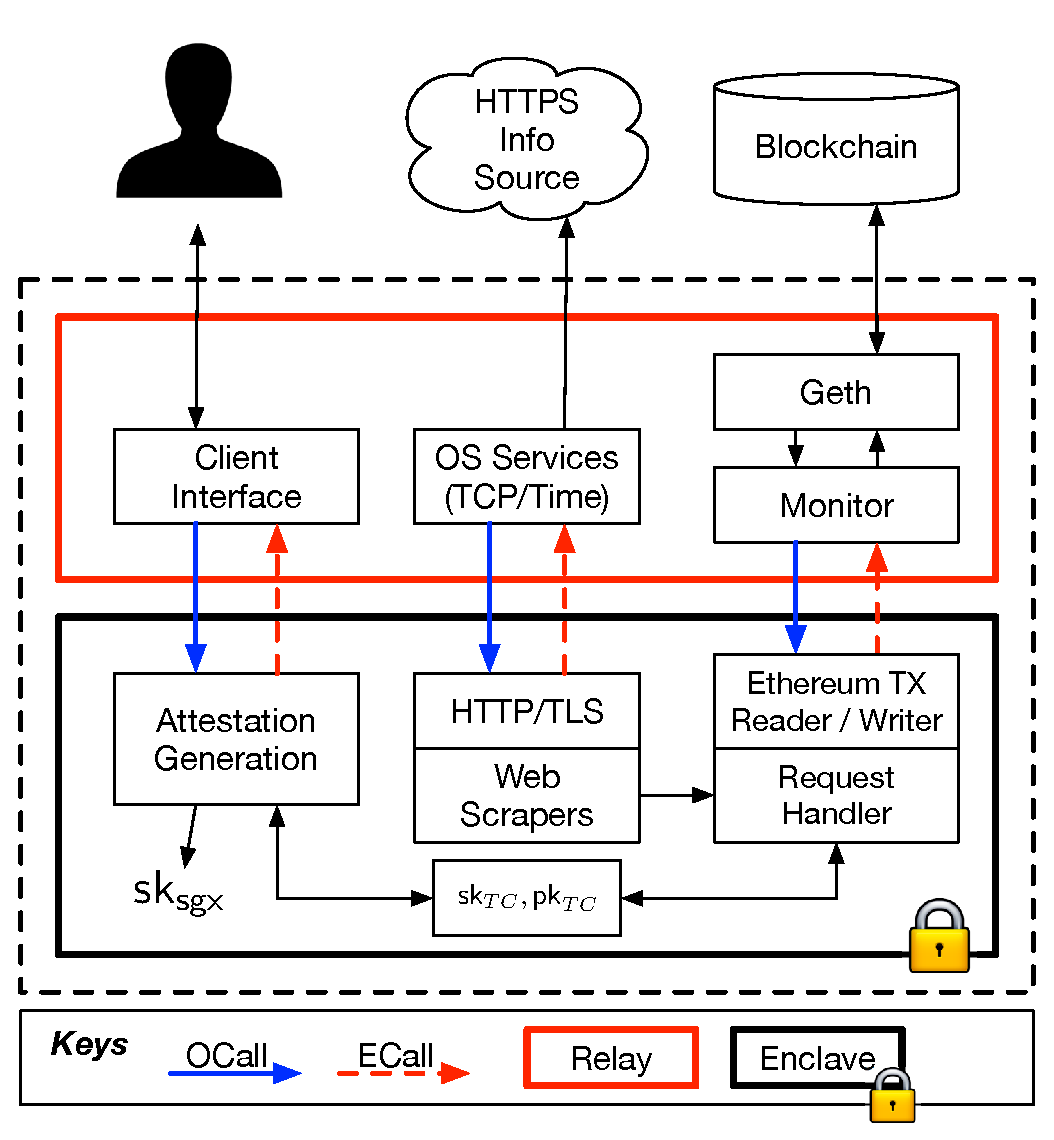
\includegraphics[width=0.45\textwidth]{figures/impl}

\begin{tikzpicture}
  [box/.style={entity, text width=1.5cm, inner sep=5pt},
   untrusted/.style={fill=red!33},
   double/.style={rectangle split, rectangle split parts=2},
   ecall/.style={color=blue,thick},
   ocall/.style={color=red!80!black,thick}]
  \matrix (m) [row sep=1.2em, column sep=0.6em]{
    \node[inner sep=0pt,anchor=south] (user) {
\includegraphics[width=1cm]{figures/user.eps}}; &
    \node[inner sep=0pt,draw,cloud,aspect=2.0,align=center,anchor=south](cloud) {\footnotesize HTTPS \\ websites}; &
    \node[box, cylinder, shape border rotate=90, aspect=.2,anchor=south](bc){blockchain};  \\[0.9em]

    \node[box,fill=white] (client) {Client \\ Interface}; & 
    \node[box,fill=white] (net) {TCP}; & 
    \node[box,fill=white,double,text width=2cm] (monitor) {\texttt{geth} \nodepart{second}{Blockchain \\ Interface}}; \\[0.6em]

    \node[box] (att) {Attestation \\ Generation}; &
    \node[box,double] (https) {HTTPS \nodepart{second}{Web \\ Scrapers}}; &
    \node[box,double,text width=2cm,] (req h){Ethereum TX \\ Reader/Writer \nodepart{second}{Request Handler}}; \\

    & \node[box,text width=2cm] (keys) {\pkTC, \skTC}; & \\
  };
  \node[anchor=west] (sk) at (keys.west-|att.west) {\skM};

  \draw[<->,thick] (user) -- (client);
  \draw[<->,thick] (net) -- (cloud);
  \draw[<->,thick] (monitor) -- (bc);

  \draw[->,ocall,transform canvas={xshift=-2mm}] (https) to (net);
  \draw[->,ocall,dashed,transform canvas={xshift=+2mm}] (net) to (https);

  \draw[->,ecall,transform canvas={xshift=-2mm}] (client) -- (att);
  \draw[<-,ecall,dashed,transform canvas={xshift=+2mm}] (client) -- (att);

  \draw[->,ecall,transform canvas={xshift=-2mm}] (monitor) -- (req h);
  \draw[<-,ecall,dashed,transform canvas={xshift=+2mm}] (monitor) -- (req h);

  \draw[<->,thick] (https.two east) -- (https.two east -| req h.two west);

  \draw[->,thick] (req h.south) |- (keys.east);
  \draw[->,thick] ([xshift=1.25em]att.south)  |- (keys.west);
  \draw[->,thick] (att.south-|sk.north) -- (sk);

  \begin{pgfonlayer}{background}
    \node [bg-box, inner sep=1.2em, tc-server-color, fit=(client)(monitor)(keys)] {};
    \node [inner sep=0.6em, untrusted, fit=(client) (net) (monitor)] {};
    \node [inner sep=0.6em, trusted, fit=(att) (https) (req h) (keys)] {};
  \end{pgfonlayer}

    \matrix (legend) [below=1.2em of m, matrix of nodes, column sep=0.75em, align=center]
  {
    \node[inner xsep=0] {\small \bf Legend:}; &
    \node[untrusted] (relay-leg) {\small Relay\vphantom{Ry}}; &
    \node[trusted] (enc-leg) {\small Enclave\vphantom{Ry}}; &
    \node[tc-server-color,rounded corners,text width=2.5em] (server-leg) {\small Server\vphantom{Ry}}; &
    \node[text width=1.75em] (ecall-leg) {}; &
    \node[text width=1.75em] (ocall-leg) {}; \\
  };

  \path[->,ecall,above] (ecall-leg.west) edge node {\small ecall} (ecall-leg.east);
  \path[<-,ecall,dashed,transform canvas={yshift=-0.4em}] (ecall-leg.west) edge (ecall-leg.east);

  \path[->,ocall,above] (ocall-leg.west) edge node {\small ocall} (ocall-leg.east);
  \path[<-,ocall,dashed,transform canvas={yshift=-0.4em}] (ocall-leg.west) edge (ocall-leg.east);
\end{tikzpicture}
\caption{Components of \tc Server}
\label{fig:tcserver_impl}
\end{figure}

For \tc, we recall that Fig.~\ref{fig:engineprotocol} shows the \encname code
$\engine$. Fig.~\ref{fig:relayprotocol} specifies the operation of the \medname,
the untrusted code in \tc, which we emphasize again provides essentially only
network functionality. We now give details on the services in the \encname and
the \medname and describe their interaction, as summarized in
Fig.~\ref{fig:tcserver_impl}.

\paragraph{\bf The \encname.} There are three components to the enclave code
\engine: An HTTPS service, Web Scrapers, which interact with data sources, and a
Request Handler, which services datagram requests. 

\vspace{2mm}

\noindent\emph{HTTPS Service.} We recall that the enclave does not have direct
access to host network functionality. \tc thus partitions HTTPS into a trusted
layer, consisting of HTTP and TLS code, and an untrusted layer that provides
low-layer network service, specifically TCP.  This arrangement allows the
enclave to establish a secure channel with a web server: The enclave itself
performs the TLS handshake with a target server and performs all cryptographic
operations internally, while the untrusted process acts as a network interface
only. We ported a TLS library (mbedTLS) into the SGX environment, as well as
HTTP code, which we minimized to meet the web-scraping requirements of \tc while
keeping the TCB small. To verify certificates presented by remote servers, we
hardcoded a collection of root CA certificates into the enclave code; in the
first version of \tc, the root CAs are identical to those in Chrome~\cite{}. By using its internal, trusted wall-clock time, it is possible to verify that a certificate has not expired. (We briefly discuss revocation in Appendix~\ref{sec:future}.)

\vspace{2mm}

\noindent\emph{Web Scrapers.} We implemented scrapers for our examples in Section~\ref{sec:applications} in an ad hoc manner for our initial implementation of \tc, and defer more principled, robust approaches to future work. 

\vspace{2mm}

\noindent\emph{Request Handler.} The Request Handler has two jobs: (1) Ingesting
a datagram request by parsing it in the serialization format specified by
Ethereum, decrypting it (if it's a private-datagram request), and dispatching
its parameters to the right scraper; and (2) Returning the response to the
request by generating an Ethereum transaction containing the requested datagram
(and parameters), serializing it as a blockchain transaction, and signing it
using \skTC. We implemented the Ethereum ABI and RLP, which respectively specify
the serialization of arguments and transactions in Ethereum. 

\vspace{2mm}

\noindent\emph{Attestation Generation.} Recall in Section \ref{sec:background}
we mentioned that an \emph{attestation} is an \emph{report} digitally signed by
the Intel-provided Quoting Enclave (QE).  Therefore two phases are involved in
generating \att. First, the \encname calls \texttt{sgx\_create\_report} to
generate a report with QE as the target enclave. Then the \medname forwards the
report to QE and calls \texttt{sgx\_get\_quote} to get a signed version of the
report, namely an attestation.

\paragraph{The \medname.} The \medname encompasses three components: A Client Interface, which serves attestations and timestamps, OS services, including networking and time services, and a Blockchain Interface. 

\vspace{2mm}

\noindent\emph{Client Interface.} As described in Section \ref{sec:architecture},
a client starts using \tc by requesting and verifying an attestation \att and checking the correctness of the clock in the \tc enclave using a fresh timestamp.
The Client Interface caches \att upon initialization of \engine. When it receives a web request from a client for an attestation,
it issues an ecall to the enclave to obtain a
Unix timestamp signed using \skTC, which it returns to the client along with \att. The client verify \att 
using the Intel Attestation Service (IAS)~\cite{} and then verify the timestamp using $\pkTC$ and check it using any trustworthy time service. 

\vspace{2mm}

\noindent\emph{OS services.} The \encname relies on the \medname to access networking and 
wall-clock time provided by the OS and implemented as ocalls.

\vspace{2mm}

\noindent\emph{Blockchain Interface.} The \medname's Blockchain Interface monitors the
blockchain for incoming requests and places transactions on the blockchain in order to
deliver datagrams. The Blockchain Interface incorporates an 
official Ethereum client, Geth~\cite{geth}. This Geth client can be configured with a JSON RPC server.  
The \medname  communicates with the blockchain indirectly via RPC calls to this server. For example, to insert a signed transaction, the \medname simply calls
\texttt{eth\_sendRawTransaction} with the byte array of the serialized
transaction. We emphasize that as the enclave holds \skTC, transactions are signed within the enclave.


%**** COLORS *********
\definecolor{maroon}{RGB}{178, 34, 34}
%\definecolor{brown}{RGB}{139, 137, 137}
\definecolor{gold}{rgb}{0.85, 0.65, 0.13}
\definecolor{darkgreen}{rgb}{0,0.5,0}
\definecolor{darkblue}{rgb}{0, 0, 0.5}

%\newcommand{\smaroon}[1]{{\ensuremath{\tt {\color{maroon} #1}\xspace}}}
%\newcommand{\sgold}[1]{\ensuremath{\tt {\color{gold} #1 \xspace}}}
%\newcommand{\sbrown}[1]{\ensuremath{\tt {\color{brown} #1 \xspace}}}

%\newcommand{\sgray}[1]{{\color{gray} #1}}

\newcommand{\ucstring}[1]{{\color{black} #1}}

\section{More Details on Formal Modeling} 
\subsection{SGX Formal Modeling}
\label{sec:sgxmodel}


As mentioned earlier, we adopt the 
UC model of SGX proposed by Shi et al.\elaine{cite}
In particular, their 
abstraction captures a subset of the features 
of Intel SGX. 
%The model follows the UC and GUC paradigm~\cite{uc,guc,juc}.
%In this paper, we use the same formal abstraction
%to model SGX (see Figure~\ref{fig:fsgx}).
%\elaine{explain more here, we can think of fsgx as a trusted third party.}
The main idea behind the UC modeling by Shi et al.
\elaine{cite}
is to think of SGX 
as a trusted third party defined by 
a global functionality $\fsgx$ (see Figure~\ref{fig:fsgx} of 
Section~\ref{sec:useofsgx}).
%In this paper, the SGX features we need include the following:

\paragraph{Modeling choices.}
For simplicity, the $\fsgx$ model currently does not 
capture the issue of revocation.
In this case, as Shi et al. point out, 
we can model SGX's group signature
simply as a regular signature scheme $\sigsgx$, whose
public and secret keys 
are called ``manufacturer keys'' and denoted $\pkM$ and $\skM$ 
(i.e., think of always signing 
with the 0-th key of the group signature scheme).
We adopt this notational choice from Shi et al. \elaine{cite} 
for simplicity. Later when 
we need to take revocation into account,
it is always possible to replace this signature 
scheme with a group signature scheme in the modeling.

The $\fsgx(\sigsgx)$ functionality described by Shi et al. \elaine{cite}
is a global functionality shared by all protocols, parametrized
by a signature scheme $\sigsgx$.
This global \fsgx 
is meant to capture all SGX machines available in the world,
and keeps track of 
multiple execution contexts
for multiple enclave programs, happening on different SGX machines in the world.
For convenience, 
this paper adopts a new notation
%In Figure~\ref{fig:fsgx}
$\fsgx(\sigsgx)[\enclaveprog, \relay]$
to denote 
one specific execution context of the global \fsgx
functionality where the enclave program in question is $\enclaveprog$,
and the specific SGX instance is attached to a physical machine $\relay$.
This specific context 
$\fsgx(\sigsgx)[\enclaveprog, \relay]$
ignores all parties' inputs except those coming from $\relay$.
We often omit writing $(\sigsgx)$ without risk of ambiguity.


\paragraph{Operations.}
$\fsgx$ captures the following features:
\begin{itemize}[leftmargin=5mm]
\item
{\it Initialize.}
Initialization is run only once.
Upon initialization, $\fsgx$
runs the initialization part of the enclave program
denoted ${\sf outp} := \enclaveprog.{\bf Initialize}()$.
Then, $\fsgx$ 
attests to the code of the enclave program $\enclaveprog$ 
%in Figure~\ref{fig:fsgx}
as well as ${\sf outp}$.
The resulting attestation is denoted 
$\sigatt$.
\item
{\it Resume.}
When \ucstring{``resume''} is invoked,
\fsgx 
calls $\enclaveprog.{\bf Resume}$
on the input parameters denoted ${\sf params}$.
$\fsgx$ 
outputs whatever $\enclaveprog.{\bf Resume}$ outputs.
\fsgx is stateful, i.e., allowed to carry state
between \ucstring{``initialize''} and multiple \ucstring{``resume''}
invocations.
\end{itemize}

Finally, we remark that this formal model by Shi et al.
is speculative,   
%Although Shi et al. propose
%a likely \fsgx abstraction, 
since we know of no formal
proof that Intel's SGX does securely realize this abstraction (or 
realize any formal
abstraction at all for that matter) --- 
in fact, available public documentations of SGX
does not provide sufficient information for making such formal proofs. 
As such, the formal model by Shi et al. 
appears to be the best available tool for us to 
formally reason about 
security 
for SGX-based protocols. 
Shi et al. leave it as an open question to design secure processors
with clear formal specifications, such that 
they can be used in the design of larger protocols/systems 
supporting formal reasoning of security.
We refer the readers to Shi et al.  \elaine{cite} for a
more detailed description of the UC modeling of Intel SGX.


\subsection{Blockchain Formal Modeling}
\label{sec:blockchainmodel}


\section{Proofs of Security Analysis}
\label{sec:analysis-proofs}

This section contains the proofs of the theorems we stated in Section~\ref{sec:analysis}


\begin{proof}[Authenticity (sketch)]
We show that if the 
adversary $\algA$ succeeds in a forgery with non-negligible probability,
we can construct an adversary $\algB$ that can either
break $\sigsgx$ or $\Sigma$ with non-neligible probability.
We consider two cases. 
The reduction $\algB$ will flip a random coin to guess which
case it is, and if the guess is wrong, simply abort.
\begin{itemize}[leftmargin=5mm]
\item
Case 1: $\algA$ outputs a signature $\sigma$ that uses the same  
$\pksgx$ as the SGX functionality $\fsgx$.
In this case, $\algB$ will try to break $\Sigma$. 
$\algB$ interacts with a signature challenger ${\sf Ch}$ who generates
some $(\pk^*, \sk^*)$ pair, and gives to $\algB$ the public key
$\pk^*$. $\algB$ simulates 
$\fsgx$ by implicitly letting $\pksgx := \pk^*$.
Whenever $\fsgx$ needs to sign a query, $\algB$ passes the signing query
onto the signature challenger ${\sf Ch}$.

Since ${\sf data} \neq \enclaveprog({\sf params})$,
$\algB$ cannot have queried ${\sf Ch}$  
on a tuple of the form $(\_, {\sf params}, {\sf data})$. 
Therefore, $\algB$ simply outputs 
what $\algA$ 
outputs (suppressing unnecessary terms) as the signature forgery. 

\item
Case 2:
 $\algA$ outputs a signature $\sigma$ that uses a different 
$\pksgx$ as the SGX functionality $\fsgx$.
In this case, $\algB$ will seek to break $\sigsgx$.
$\algB$ interacts with a signature challenger ${\sf Ch}$, who generates
some $(\pk^*, \sk^*)$ pair, and gives to $\algB$ the public key
$\pk^*$. $\algB$ simulates $\fsgx$ by implicitly setting
$\pkM := \pk^*$.
Whenever $\fsgx$ needs to make a signature
with $\skM$, 
$\algB$ simply passes the signature query onto ${\sf Ch}$.
In this case, in order for $\algA$ to succeed,
it must produce a valid signature $\sigatt$ 
for a different public key $\pk'$.
Therefore, $\algB$ simply outputs this as a signature forgery.
\end{itemize}
\end{proof}


\begin{proof}[Proof of Gas neutrality for Town Crier (sketch)]
\ethan{This needs to be redone more formally to include references to specific lines in the protocol and what they mean.
I'm going to work on that soon (probably after I eat some food...I'm hungry.}
%Honest relay means $\resumecall(\dgid, \dgform)$ will always be legitimate and $\dgform = \dgform'$ in {\bf Deliver}.
%While $\fee$ is specified by a potentially malicious user, \tcont rejects the request unless $\constgasmin \leq \fee \leq \constgasmax$.
%This means $\gasdeliver = \constgasmax \geq \fee$.
%We also will never respond to the same request twice (these are specified in the enclave protocol).
%This means that ${\sf isDelievered}[\dgid]$ will always be unset and we will always successfully retrieve a stored tuple and not abort.
%From here we consider two cases.
%
%\paragraph{Deliver called before Cancel.}
%In this case {\bf Deliver} calls $\dgcallback$ with a gas limit $\gascallback$ of $\fee - \constgasmin$ (which must be positive because of the check in {\bf Request}).
%$\constgasmin$ is set so that it is no less than the gas cost of {\bf Deliver} not including $\dgcallback$.
%That means that the total gas spent for {\bf Deliver} will be no greater than $\constgasmin + (\fee - \constgasmin) = \fee$, which is exactly what $\tcadd$ is sent for reimbursement.
%Moreover, the gas limit provided to {\bf Deliver} must be high enough because $\fee \leq \constgasmax = \gasdeliver$, so we cannot run out of gas.
%Finally, because $\fee$ was deposited with {\bf Request} and neither {\bf Deliver} nor {\bf Cancel} have been called before for this request, there must be at least $\fee$ stored $\tcont$.
%
%\paragraph{Deliver called after Cancel.}
%In this case $\tcadd$ is sent $\constgascancel$ and performs only operations of known cost.
%Because $\constgascancel$ is explicitly set to be the cost of those operations, this reimburses $\tcadd$ properly.
%Since $\fee$ was deposited with {\bf Request}, the first call to {\bf Cancel} leaves $\constgasmax$ associated with that request and subsequent calls do nothing,
%and {\bf Deliver} has not been called before for this request, there must be at least $\constgasmax$ left in $\tcont$ to send.
\end{proof}





\begin{proof}[Proof of Fair Expenditure for Honest Requester (sketch)]
$\reqcont$ is honest, so she will spend $\constgasrequest$ to invoke {\bf Request}$(\dgform, \dgcallback, \consthonestfee)$.
Ethereum does not allow money to change hands without the payer explicitly sending money.
Therefore we must only examine the explicit function invocations and monetary transfers initiated by $\reqcont$ in connection with the request.
It is impossible for $\reqcont$ to lose more money than she gives up in these transactions even if \tc is malicious.

\paragraph{Request Delivered.}
If the line marked $(\dagger)$ in Fig.~\ref{tbl:gas-tc-contract} is reached,
then we are guaranteed that $\dgform = \dgform'$ and $\gasdeliver \geq \consthonestfee$.
By Theorem~\ref{thm:authenticity}, the datagram must therefore be authentic for $\dgform$.
Because $\consthonestfee$ is chosen honestly for $\dgcallback$, $\consthonestfee - \constgasmin$ is enough gas to execute $\dgcallback$,
so $\dgcallback$ will be invoked with a datagram that is a valid and matches the request parameters.

In this case, the honest requester will have spent $\constgasrequest$ to invoke {\bf Request} and $\consthonestfee$ in paying \tc's cost for {\bf Deliver}.
The requester may have also invoked {\bf Cancel} at most once at the cost of $\constgasinvokecancel$.
While $\reqcont$ may not receive any refund due to {\bf Cancel} aborting, $\reqcont$ will still have spent at most $\constgasrequest + \constgasinvokecancel + \consthonestfee$.


\paragraph{Request not Delivered.}
If the line marked $(\ddagger)$ is reached, then $\reqcont$ will have spent
$\constgasrequest + \consthonestfee$ while executing {\bf Request},
and spent $\constgasinvokecancel$ and retrieved $\consthonestfee - \constgascancel$ while executing {\bf Cancel}.
This means the total expenditure in this case will be
\begin{align*}
  \constgasrequest + \constgasinvokecancel & + \consthonestfee - (\consthonestfee - \constgascancel) \\
                                           & = \constgasrequest + \constgasinvokecancel + \constgascancel.
\end{align*}
\end{proof}


\section{Applications and Code Samples}
\label{sec:applicationsfull}

We now elaborate 
on the applications described 
in Section~\ref{sec:applications}
and we show a short 
Solidity code sample for one of these applications,
to demonstrate first-hand what a requester  
contract would look like 
to call Town Crier's authenticated data feed service.

%We built and implemented several showcase applications.
%We give a description of these applications in this section,
%and show experimental results in Section~\ref{sec:experiments}.

\paragraph{Financial derivative ({\sf CashSettledPut}).}
Financial derivatives are among the most commonly cited smart contract
applications,
and exemplify the need for a data feed on financial instruments.
We implemented an example contract {\sf CashSettledPut} for a {\em cash-settled put option}.
This is an agreement for one party to buy an asset from the other at an agreed upon price on or before a particular date.
It is ``cash-settled'' in that the sale is implicit, i.e. no asset changes hands, only cash reflecting the asset's value.
In our implementation, the issuer of the option specifies a strike price $P_S$, expiration date, unit price $P_U$, and maximum number of units $M$ she is willing to sell.
A customer may send a request to the contract specifying the number $X$ of option units to be purchased and containing the associated fee ($X \cdot P_U$).
A customer may then exercise the option by sending another request prior to the expiration date.
{\sf CashSettledPut} calls \tc to retrieve the closing price $P_C$ of the underlying instrument on the day the option was exercised, and pays the customer $X \cdot (P_S - P_C)$.
To ensure sufficient funding to pay out, the contract must be endowed with ether value at least $M \cdot P_S$.

In Figure~\ref{fig:cash-settled-put} we describe the protocol for {\sf CashSettledPut}.
We omit the full source code due to length and complexity.

\begin{figure}[h!]
\begin{tabularx}{\linewidth}{|r@{\hspace{1ex}}X|}
  \hline

  \multicolumn{2}{|c|}{\bf {\sf CashSettledPut} blockchain contract} \\[1ex]

  \multicolumn{2}{|l|}{\bf Constants} \\
  $T_\text{stock}$ & := \tcs stock info request type \\
  $\sblue{\$F_\text{\tc}}$ & := fee payed to \tc for datagram delivery \\[1ex]

  \multicolumn{2}{|l|}{\bf Functions} \\
      {\bf Init:} & On recv $(\tcont, {\sf ticker}, P_S, P_U, M, {\sf expr}, \fee)$ from $\wallet_\text{issuer}$ \\
                  & Assert $\fee = (P_S - P_U) \cdot M + \sblue{\$F_\text{\tc}}$ \\
                  & Save all inputs and $\wallet_\text{issuer}$ to storage. \\[1ex]

      {\bf Buy:} & On recv $(X, \fee)$ from $\userwallet$: \\
                 & Assert {\sf isRecovered} not set \\
                 & \quad and ${\sf timestamp} < {\sf expr}$ \\
                 & \quad and $\wallet_\text{buyer}$ not set \\
                 & \quad and $X \leq M$ \\
                 & \quad and $\fee = (X \cdot P_U)$ \\
                 & Set $\wallet_\text{buyer} = \userwallet$ \\
                 & Save $X$ to storage \\
                 & Send $(P_S - P_U)(M - X)$ to $\wallet_\text{issuer}$ \\[-0.8em]
                 & \sgray{\it //~Hold $P_S \cdot X + \sblue{\$F_\text{\tc}}$} \\[1ex]

      {\bf Put:} & On recv $()$ from $\wallet_\text{buyer}$: \\
                 & \quad and ${\sf timestamp} < {\sf expr}$ \\
                 & \quad and ${\sf isPut}$ not set \\
                 & Set {\sf isPut} \\
                 & $\dgform := [T_\text{stock}, {\sf ticker}]$ \\
                 & $\dgcallback := {\tt this}.{\bf Settle}$ \\
                 & $\tcont.{\bf Request}(\dgform, \dgcallback, \sblue{\$F_\text{\tc}})$ \\[1ex]

   {\bf Settle:} & On recv $(\dgid, P)$ from $\tcont$: \\
                 & If $P \geq P_S$ \\
                 & \quad Send $P_S \cdot X$ to $\wallet_\text{issuer}$ \\
                 & \quad Return \\
                 & Send $(P_S - P) X$ to $\wallet_\text{buyer}$ \\
                 & Send all money in contract to $\wallet_\text{issuer}$ \\[0.25em]
                 & Send $P \cdot X$ to $\wallet_\text{issuer}$ \\[1ex]

  {\bf Recover:} & On recv $()$ from $\wallet_\text{issuer}$: \\
                 & \quad and {\sf isPut} not set \\
                 & \quad and {\sf isRecovered} not set \\
                 & \quad and $(\wallet_\text{buyer} \text{ not set}$ \\
                 & \quad \hphantom{and } or ${\sf timestamp} \geq {\sf expr})$ \\
                 & Set {\sf isRecovered} \\
                 & Send all money in contract to $\wallet_\text{issuer}$ \\[0.25em]

  \hline
\end{tabularx}
\caption{The {\sf CashSettledPut} application contract}
\label{fig:cash-settled-put}
\end{figure}



\paragraph{Flight insurance ({\sf FlightIns}).}
Flight insurance indemnifies a purchaser should her flight be delayed or canceled.
We have implemented a simple flight insurance contract called {\sf FlightIns}.
Our implementation showcases \tc's {\it private-datagram} feature to address an obvious concern:
customers may not wish to reveal their travel plans publicly on the blockchain. 

An insurer stands up {\sf FlightIns} with a specified policy fee, payout, and lead time $\Delta T$. ($\Delta T$ is set large enough to ensure that a customer can't anticipate flight cancellation or delay due to weather, etc.) To purchase a policy, a customer sends the {\sf FlightIns} a ciphertext  $C$ under the \tc's pubic key $\pkTC$ of the ICAO flight number $FN$ and scheduled time of departure $T_D$ for her flight, along with the policy fee. {\sf FlightIns} sends \tc a private-datagram request containing the current time $T$ and the ciphertext $C$. \tc decrypts $C$ and checks that the lead time meets the policy requirement, i.e., that $T_D - T \geq \Delta T$. \tc then scrapes a flight information data source several hours after $T_D$ to check the flight status, and returns to {\sf FlightIns} predicates on whether the lead time was valid and whether the flight has been delayed or canceled. If both predicates are true, then {\sf FlightIns} returns the payout to the customer. Note that $FN$ is never exposed in the clear.

Despite the use of private datagrams, {\sf FlightIns} as described here still poses a privacy risk, as the {\em timing} of the predicate delivery by \tc leaks information about $T_D$, which may be sensitive information; this, and the fact that the payout is publicly visible, could also indirectly reveal $FN$. {\sf FlightIns} addresses this issue by including in the private datagram request another parameter $t > T_D$ specifying the time at which predicates should be returned. By randomizing $t$ and making $t - T_D$ sufficiently large, {\sf FlightIns} can substantially reduce the leakage of timing information. 

In Figure~\ref{fig:flight-ins-real} we include a full implementation of {\sf FlightIns} in Solidity.

\begin{figure*}[p!]
  \centering
  \lstinputlisting[style=Solidity]{FlightIns.sol}
  \caption{Solidity code for the {\sf FlightIns} application contract.}
  \label{fig:flight-ins-real}
\end{figure*}


\paragraph{Steam Marketplace ({\sf SteamTrade}).} Steam~\cite{steam} is an online gaming platform that supports thousands of games and maintains its own marketplace, where users can trade, buy, and sell games and other virtual items.  We implement a contract for the sale of games and items for ether that showcases \tc's support for custom datagrams through the use of Steam's access-controlled API.\\
\indent A user intending to sell items creates a contract {\sf SteamTrade} with his Steam account number $ID_S$, a list $L$ of items for sale, a price $P$, and a ciphertext $C$ under the \tc's public key $\pkTC$ of his Steam API key.  In order to purchase the list of items, a buyer first uses a Steam client to create a trade offer requesting each item in $L$.  The buyer then submits to {\sf SteamTrade} his Steam account number $ID_U$, a length of time $T_U$ indicating how long the seller has to respond to the offer, and an amount of ether equivalent to the price $P$.  {\sf SteamTrade} sends \tc a custom datagram containing the current time $T$, $ID_U$, $T_U$, $L$, and the encrypted API key $C$.  \tc decrypts $C$ to obtain the API key, delays for time $T_U$, then retrieves all trades between the two accounts using the provided API key within that time period.  \tc verifies whether or not a trade exactly matching the items in $L$ successfully occurred between the two accounts and returns the result to {\sf SteamTrade}.  If such a trade occurred, {\sf SteamTrade} sends the buyer's ether to the seller's account.  Otherwise the buyer's ether is refunded.

In Figure~\ref{fig:steamtrade} we describe the protocol for {\sf CashSettledPut}.
We again omit the full source code due to length and complexity.

\begin{figure}[h!]
\begin{tabularx}{\linewidth}{|r@{\hspace{1ex}}X|}
  \hline

  \multicolumn{2}{|c|}{\bf {\sf SteamTrade} blockchain contract} \\[1ex]

  \multicolumn{2}{|l|}{\bf Constants} \\
  %$ID_S$ & := Steam account number of seller \\
  %$encAPI_S$ & := seller's encrypted API key \\
  %$List_I$ & := list of items for sale \\
  %$\sblue{\$F_\text{price}}$ & := price for listed items \\
  $T_\text{steam}$ & := \tcs Steam trade request type \\
  $\sblue{\$F_\text{\tc}}$ & := fee payed to \tc for datagram delivery \\[1ex]

  \multicolumn{2}{|l|}{\bf Functions} \\
  {\bf Init:}   & On recv $(\tcont, ID_S, encAPI_S, List_I, P)$ from $\wallet_\text{seller}$: \\
                & Save all inputs and $\wallet_\text{seller}$ to storage. \\[1ex]

  {\bf Buy:} & On recv $(ID_U, T_U, \fee)$ from $\userwallet$: \\
                & Assert $\fee = P$ \\
                & $\dgform := [encAPI_S, ID_U, T_U, LIST_I]$ \\
                & $\dgcallback := {\tt this}.{\bf Pay}$ \\
                & $\dgid := \tcont.{\bf Request}(\dgform, \dgcallback, \sblue{\$F_\text{\tc}})$ \\
                & Store $(\dgid, \userwallet)$ \\[1ex]

  {\bf Pay:}    & On recv $(\dgid, status)$ from $\tcont$: \\
                & Retrieve and remove stored $(\dgid, \userwallet)$ \\
                & \quad \sgray{\it //~Abort if not found} \\
                & If $status > 0$ \\
                & \quad Send $\sblue{\$F_\text{price}}$ to $\wallet_\text{seller}$ \\
                & Else \\
                & \quad send $\sblue{\$F_\text{price}}$ to $\userwallet$ \\
                [0.25em]

  \hline
\end{tabularx}
\caption{The {\sf FlightIns} application contract}
\label{fig:steamtrade}
\end{figure}


%Discuss flight insurance as an example: We'd like to conceal the flight number and date. We might also want to conceal payment, so TC might ingest encrypted addresses and mix them internally.

%Micro-loans too? Linkage to Facebook / Keybase.io


%\section{Future Work}
\label{sec:future}

We plan to develop \tc after its initial deployment and expect it to evolve to incorporate a number of additional features. These fall into two categories: (1) Expanding the security model to address threats outside the scope of the initial version and (2) Extending the functionality of \tc. Here we briefly discuss a few of these extensions.

\subsection{Expanding \tc threat model}

\begin{itemize}
\item{\em Freeloading protection.} Serious concerns have  arisen in the Ethereum community about ``parasite contracts'' that forward or resell datagrams---particularly those from fee-based data feeds~\cite{parasite}. We plan to deploy a novel mechanism in \tc to address this concern. Suppose contract \reqcont involves a set of parties / users $U = \{U_i\}_{i=1}^n$. Each player $U_i$ generates an individual share $(\sk_i, \pk_i)$ of a global keypair $(\pk, \sk)$, where $\sk = \sum_{i=1} \sk_i$ and $\pk = \prod_{i=1} \pk_i$, and communicates a ciphertext $E_{\pkTC}[\sk_i]$ to \tcont, e.g., by including it in a datagram request. Players then jointly set  up under public key $\pk$ a wallet $\specialwallet$ for datagram transmission by \tcont. 

Thanks to the homomorphic properties of ECDSA, \tcont can compute $\sk$ (non-interactively) and send datagrams from $\specialwallet$. But the users $U$ collaboratively \emph{can also compute $\sk$ and send messages from $\specialwallet$}. Consequently, while each user $U_i$ can individually be assured that a datagram sent to \reqcont by \tcont from $\specialwallet$ is valid (as $P[i]$ didn't collude in its creation), other players cannot determine whether a datagram was produced by $\tcont$ or $U$, and thus whether or not it is valid. Such a \emph{source-equivocal datagram} renders data from parasite contracts less trustworthy and thus less attractive. 
\item{\em Traffic-analysis protection.} As noted in the body of the paper, \medname can observe the pattern of data sources accesses made by \tc. By correlating with activity in \tcont, an adversarial \medname can thus infer the data source targeted by private datagrams, as well as the timing---and potentially, based on traffic analysis, of the \encname's HTTPS requests. (See, e.g.,~\cite{chen2010side}.) In the example contract {\sf FlightIns} in Section~\ref{sec:applications}, this issue is partially addressed through the insertion of random delays into \tc responses. We intend to develop a comprehensive approach to mitigating traffic analysis in \tc. This approach will include, for the problem of traffic analysis of web scraping, the incorporation of facilities in the \encname to make chaff or decoy data requests, i.e., false requests, to both the true data source and well as non-target data sources. 

\item{\em Revocation support.} Revocation of two forms can impact the \tc service. 

First, the certificates of data sources may be revoked. To address this issue, given its ability to establish external HTTPS connections, \tc could easily make use of Online Certificate Status Protocol (OCSP) certificate checking. This functionality would amount to an additional form of web scraping, and could be executed in parallel with web scraping to support datagram requests, resulting in minimal additional latency.

Second, an SGX host could become compromised, prompting revocation of its EPID signatures by Intel. The Intel Attestation Service (IAS) will reportedly provide support for online attestation verification and thus for revocation. Conveniently, clients use the IAS when checking the attestation $\sigatt$, so no modification to \tc is required to support the service.


\item{\em SLAs.} Were \tc to be deployed as a fee-for-service system, requesters might wish to see Service Level Agreements (SLAs) enforced. A temporary outage on a \tc host or a malicious \medname could cause a delay in datagram delivery, potentially with aftereffects in relying contracts. An SLA could be implemented as an indemnity paid to a contract if a datagram is not delivered within a specified period of time. This feature could itself be implemented, for example, as an entry point in $\tcont$. (Naturally care would be required to ensure that $\tcont$ holds funds sufficient for payout in the case of a general delivery failure.)

\item{\em Hedging against SGX compromise.} We discussed in Section~\ref{subsec:enhanced_robustness} and demonstrated in Section~\ref{subsec:hedging} how \tc can support majority voting across SGX hosts and/or data sources to hedge against failures in either (outside \tc's basic security model) via majority voting. It would be possible to reduce the latency and gas costs of such voting with design enhancements to \tc. Specifically, for the case of SGX voting, we plan to investigate a scheme in which consensus on a datagram value $X$ is reached off-chain among SGX-enable \tc hosts  via Byzantine consensus. These hosts may then use a threshold digital signature scheme to sign the datagram response from ${\cal W}_{TC}$. To ensure that the response is delivered to the blockchain, each participating host can monitor the blockchain and itself transmit the response in the case of an observed delivery failure. This approach will largely eliminate the incremental gas cost of majority voting across SGX instances.

\end{itemize}

\subsection{Expanding \tc functionality}

\begin{itemize}
\item{\em New opcodes.} Ethereum's developers~\cite{Buterinpersonal} have indicated an intention to expand the range of supported cryptographic primitives in Ethereum and stated that they are amenable to the authors' suggestion of incorporating opcodes supporting Intel's EPID in particular, which would enable efficient attestation verification within the blockchain. 
\item{\em Migration to data-source feeds.} Ultimately, we envision that data sources may wish themselves to serve as authenticated data feeds. To do so, they could simply stand up \tc as a front end. As a first step along this path, however, an independent \tc service might provide support for XML-labelled data from data sources, enabling more accurate and direct scraping and intentional identification of what data should be served. We plan to build support for such explicit data labeling into \tc should this approach prove attractive to data sources.
\item{\em Generalized custom datagrams.} In our example smart contract {\sf SteamTrade}, we demonstrated a custom datagram that is essentially hardwired: It employs a user's credentials to scrape her individual online account. A more general approach would be to allow contract owners to specify their own generalized functionalities--scrapers and/or confidential contract modules---as general purpose code, achieving a data-source-enriched emulation of private contracts as in Hawk~\cite{hawk}, but with much lower resource requirements. Furnishing large custom datagrams on the blockchain would be prohibitively expensive, but off-chain loading of code would be quite feasible. Of course, many security and confidentiality considerations arise in a system that allows users to deploy arbitrary code, giving rise to programming language challenges that deployment of this feature in \tc would need to address.
\end{itemize}



%
\section{Implementation Pseudocode}


\subsection{Application Contracts}
\label{sec:app-contract-code}


\begin{figure}[h!]
\begin{tabularx}{\linewidth}{|r@{\hspace{1ex}}X|}
  \hline

  \multicolumn{2}{|c|}{\bf {\sf FlightIns} blockchain contract} \\[1ex]

  \multicolumn{2}{|l|}{\bf Constants} \\
  $D_{\rm min}$ & := minimum delay to pay out insurance \\
  $T_\text{flight}$ & := \tcs flight info request type \\
  $\smaroon{\$F_\text{prem}}$ & := premium to buy insurance \\
  $\smaroon{\$F_\text{pay}}$ & := payout if flight is canceled or delayed \\
  $\smaroon{\$F_\text{\tc}}$ & := fee payed to \tc for datagram delivery \\[1ex]

  \multicolumn{2}{|l|}{\bf Functions} \\
  {\bf Init:}   & On recv $(\tcont)$: \\
                & Save address of \tcont \\[1ex]

  {\bf Insure:} & On recv $(encFN, \fee)$ from $\userwallet$: \\
                & Assert $\fee = \smaroon{\$F_\text{prem}}$ \\
                & $\dgform := [T_\text{flight}, encFN]$ \\
                & $\dgcallback := {\tt this}.{\bf Pay}$ \\
                & $\dgid := \tcont.{\bf Request}(\dgform, \dgcallback, \smaroon{\$F_\text{\tc}})$ \\
                & Store $(\dgid, \userwallet)$ \\[1ex]

  {\bf Pay:}    & On recv $(\dgid, D)$ from $\tcont$: \\
                & Retrieve and remove stored $(\dgid, \userwallet)$ \\
                & \quad \sgray{\it //~Abort if not found} \\
                & If $D \geq D_{\rm min}$ \\
                & \quad Send $\smaroon{\$F_\text{pay}}$ to $\userwallet$ \\[0.25em]

  \hline
\end{tabularx}
\caption{The {\sf FlightIns} application contract}
\label{tbl:flight-ins}
\end{figure}


\begin{figure}[h!]
\begin{tabularx}{\linewidth}{|r@{\hspace{1ex}}X|}
  \hline

  \multicolumn{2}{|c|}{\bf {\sf CashSettledPut} blockchain contract} \\[1ex]

  \multicolumn{2}{|l|}{\bf Constants} \\
  $T_\text{stock}$ & := \tcs stock info request type \\
  $\smaroon{\$F_\text{\tc}}$ & := fee payed to \tc for datagram delivery \\[1ex]

  \multicolumn{2}{|l|}{\bf Functions} \\
      {\bf Init:} & On recv $(\tcont, {\sf ticker}, P_S, P_U, M, {\sf expr}, \fee)$ from $\wallet_\text{issuer}$ \\
                  & Assert $\fee = (P_S - P_U) \cdot M + \smaroon{\$F_\text{\tc}}$ \\
                  & Save all inputs and $\wallet_\text{issuer}$ to storage. \\[1ex]

      {\bf Buy:} & On recv $(X, \fee)$ from $\userwallet$: \\
                 & Assert {\sf isRecovered} not set \\
                 & \quad and ${\sf timestamp} < {\sf expr}$ \\
                 & \quad and $\wallet_\text{buyer}$ not set \\
                 & \quad and $X \leq M$ \\
                 & \quad and $\fee = (X \cdot P_U)$ \\
                 & Set $\wallet_\text{buyer} = \userwallet$ \\
                 & Save $X$ to storage \\
                 & Send $(P_S - P_U)(M - X)$ to $\wallet_\text{issuer}$ \\[-0.8em]
                 & \sgray{\it //~Hold $P_S \cdot X + \smaroon{\$F_\text{\tc}}$} \\[1ex]

      {\bf Put:} & On recv $()$ from $\wallet_\text{buyer}$: \\
                 & \quad and ${\sf timestamp} < {\sf expr}$ \\
                 & \quad and ${\sf isPut}$ not set \\
                 & Set {\sf isPut} \\
                 & $\dgform := [T_\text{stock}, {\sf ticker}]$ \\
                 & $\dgcallback := {\tt this}.{\bf Settle}$ \\
                 & $\tcont.{\bf Request}(\dgform, \dgcallback, \smaroon{\$F_\text{\tc}})$ \\[1ex]

   {\bf Settle:} & On recv $(\dgid, P)$ from $\tcont$: \\
                 & If $P \geq P_S$ \\
                 & \quad Send $P_S \cdot X$ to $\wallet_\text{issuer}$ \\
                 & \quad Return \\
                 & Send $(P_S - P) X$ to $\wallet_\text{buyer}$ \\
                 & Send all money in contract to $\wallet_\text{issuer}$ \\[0.25em]
                 & Send $P \cdot X$ to $\wallet_\text{issuer}$ \\[1ex]

  {\bf Recover:} & On recv $()$ from $\wallet_\text{issuer}$: \\
                 & \quad and {\sf isPut} not set \\
                 & \quad and {\sf isRecovered} not set \\
                 & \quad and $(\wallet_\text{buyer} \text{ not set}$ \\
                 & \quad \hphantom{and } or ${\sf timestamp} \geq {\sf expr})$ \\
                 & Set {\sf isRecovered} \\
                 & Send all money in contract to $\wallet_\text{issuer}$ \\[0.25em]

  \hline
\end{tabularx}
\caption{The {\sf CashSettledPut} application contract}
\label{tbl:cash-settled-put}
\end{figure}


\begin{figure}[h!]
\begin{tabularx}{\linewidth}{|r@{\hspace{1ex}}X|}
  \hline

  \multicolumn{2}{|c|}{\bf {\sf SteamTrade} blockchain contract} \\[1ex]

  \multicolumn{2}{|l|}{\bf Constants} \\
  %$ID_S$ & := Steam account number of seller \\
  %$encAPI_S$ & := seller's encrypted API key \\
  %$List_I$ & := list of items for sale \\
  %$\smaroon{\$F_\text{price}}$ & := price for listed items \\
  $T_\text{steam}$ & := \tcs flight info request type \\
  $\smaroon{\$F_\text{\tc}}$ & := fee payed to \tc for datagram delivery \\[1ex]

  \multicolumn{2}{|l|}{\bf Functions} \\
  {\bf Init:}   & On recv $(\tcont, ID_S, encAPI_S, List_I, P)$ from $\wallet_\text{seller}$: \\
                & Save all inputs and $\wallet_\text{seller}$ to storage. \\[1ex]

  {\bf Purchase:} & On recv $(ID_U, T_U, \fee)$ from $\userwallet$: \\
                & Assert $\fee = P$ \\
                & $\dgform := [encAPI_S, ID_U, T_U, LIST_I]$ \\
                & $\dgcallback := {\tt this}.{\bf Pay}$ \\
                & $\dgid := \tcont.{\bf Request}(\dgform, \dgcallback, \smaroon{\$F_\text{\tc}})$ \\
                & Store $(\dgid, \userwallet)$ \\[1ex]

  {\bf Pay:}    & On recv $(\dgid, status)$ from $\tcont$: \\
                & Retrieve and remove stored $(\dgid, \userwallet)$ \\
                & \quad \sgray{\it //~Abort if not found} \\
                & If $status > 0$ \\
                & \quad Send $\smaroon{\$F_\text{price}}$ to $\wallet_\text{seller}$ \\
                & Else \\
                & \quad send $\smaroon{\$F_\text{price}}$ to $\userwallet$ \\
                [0.25em]

  \hline
\end{tabularx}
\caption{The {\sf FlightIns} application contract}
\label{tbl:steamtrade}
\end{figure}




%\theendnotes
\end{document}
